%!TeX document-id = {bff9011c-8ff8-4be2-916a-5647c89bca22}
%!TeX program = pdflatex
%!TeX TXS-program:compile = txs:///pdflatex | txs:///biber | txs:///pdflatex
%!TeX TXS-program:bibliography = txs:///biber
%!BIB TS-program = biber
%======================================================================
%	
%	 __  __       _         ______ _ _      
%	|  \/  |     (_)       |  ____(_) |     
%	| \  / | __ _ _ _ __   | |__   _| | ___ 
%	| |\/| |/ _` | | '_ \  |  __| | | |/ _ \
%	| |  | | (_| | | | | | | |    | | |  __/
%	|_|  |_|\__,_|_|_| |_| |_|    |_|_|\___|
%
%----------------------------------------------------------------------
% Descripton : Main File to compose the resulting PDF
%======================================================================
% Wichtig um die Bibliography zu compilen bitte einfach einmal F8 und danach nochmal normal Compilen!!!
% oder in TeXStudio unter Optionen -> Erzeugen -> und Dann die Sequenz pdfLatex -> Biber -> pdfLatex
% oder einfach F5 -> F8 -> F5
%======================================================================
% Beim Fehler 
% 	TeX capacity exceeded, sorry [main memory size=3000000].....
% Folgendes verwenden 
% https://tex.stackexchange.com/questions/7953/how-to-expand-texs-main-memory-size-pgfplots-memory-overload
% also pdflatex ... --extra-mem-top=10000000 .... <filename> bei TeXStudio ersetzen!
%======================================================================
%\pdfobjcompresslevel=0
\pdfminorversion=7
\pdfinclusioncopyfonts=1
\documentclass[
				%ngerman            % neue deutsche Rechtschreibung
				,a4paper            % Papiergrösse
				,twoside            % Zweiseitiger Druck (rechts/links)
				% ,10pt             % Schriftgrösse
				,11pt
				% ,12pt
				,pdftex
				% ,disable         % Todo-Markierungen auschalten
				,notitlepage		% Thanks abstract... preventing it from removing pageNumber
				]{report}

% Bitte die Codierung Ihrer Dateien auswählen:
% \usepackage[latin1]{inputenc}    % Für UNIX mit ISO-LATIN-codierten Dateien
% \usepackage[applemac]{inputenc}  % Für Apple Mac
% \usepackage[ansinew]{inputenc}   % Für Microsoft Windows
\usepackage[utf8]{inputenc}        % UTF-8 codierte Dateien
% Dieses Dokument ist unter Unix erstellt, daher
% wird diese Input-Codierung benutzt.

%————————————————————————————————————————————————————————————————————————————
%					Import aller Konfigurationen
%————————————————————————————————————————————————————————————————————————————
\usepackage{./config/DHBW/bericht}
\usepackage{./config/PaketeProjektarbeit} % <- spezifische Pakete für die Projektarbeit
\usepackage{./config/Pakete}
\usepackage{./config/Befehle}
\usepackage{./config/Layout}
\usepackage{./config/Styles}
%Wenn PDF/A-1B gewünscht .. Achtung am besten nochmal mit veraPDF testen!
\usepackage{./config/PDFStandard}

%————————————————————————————————————————————————————————————————————————————
%					Variablen deklarieren
%————————————————————————————————————————————————————————————————————————————
%======================================================================
%	
%	__      __        _       _     _            
%	\ \    / /       (_)     | |   | |           
%	 \ \  / /_ _ _ __ _  __ _| |__ | | ___ _ __  
%	  \ \/ / _` | '__| |/ _` | '_ \| |/ _ \ '_ \ 
%	   \  / (_| | |  | | (_| | |_) | |  __/ | | |
%	    \/ \__,_|_|  |_|\__,_|_.__/|_|\___|_| |_|
%
%----------------------------------------------------------------------
% Descripton : Variables
%======================================================================

\newboolean{DEBUG}
\newboolean{BERICHTE}
\newboolean{SPERRVERMERK}
\newboolean{CHANGELOG}
\newboolean{VORWORT}
\newboolean{ABSTRACT}
\newboolean{DANKSAGUNG}
\newboolean{WATERMARK}
\newboolean{INDEX}
\newboolean{TRENNSTRICHE}
\newboolean{ERKLAERUNG}
\newboolean{DOKUMENTENVERZEICHNIS}
\newboolean{DATEIVERZEICHNIS}
\newboolean{LITERATURVERWEIS}
\newboolean{DIGITALE-UNTERSCHRIFT}
\newboolean{DIGITAL-SIGN-AREA}
\newboolean{CDBEILAGE}
\newboolean{TODO}
\newboolean{BLACKOUT}

%————————————————————————————————————————————————————————————————————————————
%					Informationen ausfüllen
%————————————————————————————————————————————————————————————————————————————
%======================================================================
%	
%	_____        __                           _   _             
%  |_   _|      / _|                         | | (_)            
%	 | |  _ __ | |_ ___  _ __ _ __ ___   __ _| |_ _  ___  _ __  
%    | | | '_ \|  _/ _ \| '__| '_ ` _ \ / _` | __| |/ _ \| '_ \ 
%	_| |_| | | | || (_) | |  | | | | | | (_| | |_| | (_) | | | |
%  |_____|_| |_|_| \___/|_|  |_| |_| |_|\__,_|\__|_|\___/|_| |_|
%
%----------------------------------------------------------------------
% Descripton : File with all Information about the Document
%======================================================================

\newcommand{\Autor}{Max Mustermann}
\newcommand{\MatrikelNummer}{4711}
\newcommand{\Kursbezeichnung}{tinf17b3}

\newcommand{\FirmenName}{Firmenname}
\newcommand{\FirmenStadt}{Stadt}
\newcommand{\FirmenLogoDeckblatt}{\fbox{
\includegraphics[width=3cm]{./config/layout/firmenlogo}}}

% Falls es kein Firmenlogo gibt:
%  \newcommand{\FirmenLogoDeckblatt}{}

\newcommand{\BetreuerFirma}{Titel Vorname Nachname}
\newcommand{\BetreuerDHBW}{Titel Vorname Nachname}

%%%%%%%%%%%%%%%%%%%%%%%%%%%%%%%%%%%%%%%%%%%%%%%%%%%%%%%%%%%%%%%%%%%%%%%%%%%%%%%%%%%%%

% Wird auf dem Deckblatt und in der Erklärung benutzt:
\newcommand{\Was}{Projekt-/Studien-/Bachelorarbeit}
%\newcommand{\Was}{Projektarbeit I}
%\newcommand{\Was}{Projektarbeit II}
%\newcommand{\Was}{Projektarbeit III}
%\newcommand{\Was}{Studienarbeit}
%\newcommand{\Was}{Bachelorthesis}

%%%%%%%%%%%%%%%%%%%%%%%%%%%%%%%%%%%%%%%%%%%%%%%%%%%%%%%%%%%%%%%%%%%%%%%%%%%%%%%%%%%%%

\newcommand{\Titel}{\LaTeX-Vorlage für diverse Ausarbeitungen .. oder so ähnlich}
\newcommand{\AbgabeDatum}{1. April 2090}

\newcommand{\Dauer}{12 Wochen}

% \newcommand{\Abschluss}{Bachelor of Engineering}
\newcommand{\Abschluss}{Bachelor of Science}

\newcommand{\Studiengang}{Informatik / Informationstechnik}
% \newcommand{\Studiengang}{Informatik / Angewandte Informatik}
%======================================================================
%	 _    _                                 __ 
%	| |  | |                               / _|
%	| |__| |_   _ _ __   ___ _ __ _ __ ___| |_ 
%	|  __  | | | | '_ \ / _ \ '__| '__/ _ \  _|
%	| |  | | |_| | |_) |  __/ |  | | |  __/ |  
%	|_|  |_|\__, | .__/ \___|_|  |_|  \___|_|  
%		     __/ | |                           
%		    |___/|_|                           
%
%----------------------------------------------------------------------
% Descripton : Hyperref File for setting PDF Information
%======================================================================

\hypersetup{
	unicode=false,
	pdftoolbar=true,
	pdfmenubar=true,
	pdffitwindow=false,
	pdfstartview={FitH},
	pdftitle={\Titel},
	pdfauthor={\Autor},
	pdfsubject={\Was},
	pdfcreator={\Autor},
	pdfkeywords={DHBW},
	pdfborderstyle={/S/U/W 1},
	pdfnewwindow=true,
	citebordercolor=LimeGreen,
	filebordercolor=Magenta,
	linkbordercolor=Orange,
	menubordercolor=Orange,
	urlbordercolor=Fuchsia,
	runbordercolor=Orange
}


%————————————————————————————————————————————————————————————————————————————
%					Sonstige Einstellungen
%————————————————————————————————————————————————————————————————————————————
\addbibresource{directories/bibliography.bib}
\loadglsentries{./directories/glossary}
\makeglossaries
\makeindex[columns=1,options={-s ./config/DHBW/bericht.ist}]
%======================================================================
%                                              
%	    /\                                        
%	   /  \   ___ _ __ ___  _ __  _   _ _ __ ___  
%	  / /\ \ / __| '__/ _ \| '_ \| | | | '_ ` _ \ 
%	 / ____ \ (__| | | (_) | | | | |_| | | | | | |
%	/_/    \_\___|_|  \___/|_| |_|\__, |_| |_| |_|
% 	                              __/ |          
%	                              |___/             
%
%----------------------------------------------------------------------
% Author : Nico Holzhäuser
% Descripton : Acronyms
%======================================================================

%\chapter*{Abkürzungsverzeichnis} % chapter*{..} --> keine Nummer, kein "Kapitel"
						         % Nicht ins Inhaltsverzeichnis

\acsetup{
	list/display = used,
	pages/display = first
}

% Alle Bestandteile auf https://packages.oth-regensburg.de/ctan/macros/latex/contrib/acro/acro-manual.pdf -> Seite 7

%\DeclareAcronym{}{
%	short = SHORTFORM,			% <- required Shortform
%	long = LONGFORM,			% <- Long Form of the Acronym
%	foreign = FOREIGN			% <- Foreign Form
%	tag = acronym,				% <- Tag for printing
%	sort = SORTKEY				% <- Sort Key, if you use Math Symbols
%}


\DeclareAcronym{WWW}{
	short = WWW,
	long = World Wide Web,
	tag = acronym
}

\DeclareAcronym{Abk}{
	short = Abk.,
	long =Abkürzung,
	tag = acronym
}

\DeclareAcronym{DHBW}{
	short = DHBW,
	long = Duale Hochschule Baden-Württemberg,
	tag = acronym
}

\DeclareAcronym{H2O}{
	short = \ensuremath{H_2O},
	long = Di-Hydrogen-Monoxid,
	tag = acronym,
	sort = H20
}

\DeclareAcronym{NUA}{
	short = NUA,
	long = Not used Acronym,
	tag = acronym
}


%————————————————————————————————————————————————————————————————————————————
%					Einstellungen
%————————————————————————————————————————————————————————————————————————————
% Debug auf true setzen, hierbei wird der Changelog hinzugefügt, und keine Doppelseitenumbrüche gemacht (Zum drucken -> false)
% Bitte zum drucken oben in der Präambel auch auf Doppelseite schalten!
\setboolean{DEBUG}{true}
% Soll der Changelog angezeigt werden ?
\setboolean{CHANGELOG}{true}
% Sollen die TODO's angezeigt werden ?
\setboolean{TODO}{true}
% =================================================================================================
%Digitale Unterschrift auf die Erklärung -> PDF in zfiles/Signaturen/ und dann Signatur.pdf und Ort_Datum.pdf ??
\setboolean{DIGITALE-UNTERSCHRIFT}{true}
%Digitale Unterschriftsfeld auf die Erklärung ??
\setboolean{DIGITAL-SIGN-AREA}{false}
\ifthenelse{\boolean{DIGITAL-SIGN-AREA}}{\setboolean{DIGITALE-UNTERSCHRIFT}{false}}{}
% =================================================================================================
% Soll eine Erklärung eigefügt werden ?
\setboolean{ERKLAERUNG}{true}
%Soll das Abstract eingefügt werden ?
\setboolean{ABSTRACT}{true}
%Soll das Vorwort eingefügt werden ?
\setboolean{VORWORT}{true}
%Soll das Vorwort eingefügt werden ?
\setboolean{DANKSAGUNG}{true}
%Soll ein Sperrvermerk gemacht werden
\setboolean{SPERRVERMERK}{true}
%Literaturverweis auf Speicherung
\setboolean{LITERATURVERWEIS}{true}
% =================================================================================================
% Soll ein Index eingefügt werden ?
\setboolean{INDEX}{true}
%Soll ne Trennlinie im Inhaltsverzeichnis eingefügt werden, vor Verzeichnissen, dem Inhalt und dem Anhang
\setboolean{TRENNSTRICHE}{true}
%Setzt ein Watermark
\setboolean{WATERMARK}{false}
% =================================================================================================
%Dokumentenverzeichnis generieren ?
\setboolean{DOKUMENTENVERZEICHNIS}{true}
%Dateiverzeichnis generieren ?
\setboolean{DATEIVERZEICHNIS}{true}
% Soll auf das Dateiverzeichnis die CD ?
\setboolean{CDBEILAGE}{true}
%Sind Berichte abzugeben ? Automatische einbindung zum Drucken
\setboolean{BERICHTE}{true}

%————————————————————————————————————————————————————————————————————————————
%					Watermark
%————————————————————————————————————————————————————————————————————————————
\ifthenelse{\boolean{WATERMARK}}{\usepackage{draftwatermark}}{}
\ifthenelse{\boolean{WATERMARK}}{\SetWatermarkText{Entwurf}}{}

%————————————————————————————————————————————————————————————————————————————
%					PDF Optionen
%————————————————————————————————————————————————————————————————————————————
%Soll der Changelog angezeigt werden -- Sowieso nur im DEBUG?
\ifthenelse{\boolean{DEBUG}}{}{\setboolean{CHANGELOG}{false}}
%Package um die Referenzen zu checken, einfach im Log nach "refcheck suchen!"
%\usepackage{refcheck}

%————————————————————————————————————————————————————————————————————————————
%									Anfang Dokument
%————————————————————————————————————————————————————————————————————————————
\begin{document}
	
	% Ab hier beginnt die Seitenzählung für den Prefix in kleinen römischen Zahlen
	% Erste Seite nach der Titelseite
	\pagenumbering{roman}
	
	%—————————————————————————————————————————————————————————————————————————
	%								Deckseite
	%—————————————————————————————————————————————————————————————————————————
	\begin{titlepage}
		%%%%%%%%%%%%%%%%%%%%%%%%%%%%%%%%%%%%%%%%%%%%%%%%%%%%%%%%%%%%%%%%%%%%%%%%%%%%%%%
%% Descr:       Vorlage für Berichte der DHBW-Karlsruhe, Titlepage
%% Author:      Prof. Dr. Jürgen Vollmer, vollmer@dhbw-karlsruhe.de
%% $Id: erklaerung.tex,v 1.11 2020/03/13 14:24:42 vollmer Exp $
%% -*- coding: utf-8 -*-
%%%%%%%%%%%%%%%%%%%%%%%%%%%%%%%%%%%%%%%%%%%%%%%%%%%%%%%%%%%%%%%%%%%%%%%%%%%%%%%

\begin{center}
	\vspace*{-2cm}
	\FirmenLogoDeckblatt\hfill
\includegraphics[width=4cm]{./config/DHBW/dhbw-logo.png}\\[2cm]
	{\Huge \Titel}\\[1cm]
	{\Huge\scshape \Was}\\[1cm]
	{\large für die Prüfung zum}\\[0.5cm]
	{\Large \Abschluss}\\[0.5cm]
	{\large des Studienganges \Studiengang}\\[0.5cm]
	{\large an der}\\[0.5cm]
	{\large Dualen Hochschule Baden-Württemberg Karlsruhe}\\[0.5cm]
	{\large von}\\[0.5cm]
	{\large\bfseries \Autor}\\[1cm]
	{\large Abgabedatum \AbgabeDatum}
	\vfill
\end{center}
\begin{tabular}{l@{\hspace{2cm}}l}
	Bearbeitungszeitraum	         & \Dauer 			\\
	Matrikelnummer	                 & \MatrikelNummer		\\
	Kurs			         & \Kursbezeichnung		\\
	Ausbildungsfirma	         & \FirmenName			\\
	& \FirmenStadt			\\
	Betreuer der Ausbildungsfirma	 & \BetreuerFirma		\\
	Gutachter der Studienakademie	 & \BetreuerDHBW		\\
\end{tabular}
	\end{titlepage}
	
	%—————————————————————————————————————————————————————————————————————————
	%								Changelog
	%—————————————————————————————————————————————————————————————————————————
	\ifthenelse{\boolean{CHANGELOG}}{
		%======================================================================
%	
%	  _____ _                            _             
%	 / ____| |                          | |            
%	| |    | |__   __ _ _ __   __ _  ___| | ___   __ _ 
%	| |    | '_ \ / _` | '_ \ / _` |/ _ \ |/ _ \ / _` |
%	| |____| | | | (_| | | | | (_| |  __/ | (_) | (_| |
%	 \_____|_| |_|\__,_|_| |_|\__, |\___|_|\___/ \__, |
%						       __/ |              __/ |
%							  |___/              |___/ 
%
%----------------------------------------------------------------------
% Descripton : Changelog
%======================================================================

\chapter*{Änderungen}

\begin{description}
	\item[2022/04/05 - NH] Anpassen der Packages 
	\item[2022/02/03 - NH] Moved appendix into Pages
	\item[2022/02/03 - NH] Major Structure Refactoring - added IMRAD Schema
	\item[2022/01/17 - NH] Code-Refactoring + Fix für TODONotes + Mehr Output-Streams hinzugefügt im 
							Package
	\item[2022/01/17 - NH] Verzeichnisstruktur angepasst + Kleine Fixes
	\item[2022/01/17 - NH] Bugfix für den Trennstrich
	\item[2021/09/14 - NH] Anpassung der Seitennummern + Korrektur des Dokumentenverzeichnis
	\item[2021/09/01 - NH] Digitale Unterschrift nun möglich .. ob die DHBW das akzeptiert :-/ \\
						   Feld + Boolean für Digital Signing von Adobe eingefügt!
	\item[2021/08/23 - NH] Dokumentenverzeichnis, sowie Dateiverzeichnis hinzugefügt!
	\item[2021/08/18 - NH] PDF/A-1B Standart wird unterstützt .... JUHUUUU
	\item[2021/08/17 - NH] Fixed various Bugs with Booleans + Added own Bibliography for the Presentation!
	\item[2021/08/12 - NH] Refcheck Package eingefügt, um falsche Referenzen einfacher zu finden
	\item[2021/08/03 - NH] Hyperlinks gefixt, und Inhaltsseite eingefügt
	\item[2021/07/23 - NH] Verschiedene Formatierungen gefixt und Index eingefügt
	\item[2021/07/19 - NH] Befehl für Boxshadows eingefügt
	\item[2021/03/10 - NH] Watermark eingefügt
	\item[2020/03/13 - JV] Tippfehler korrigiert\\
	                  aktuelle Formulierungen aus der Prüfungsordnung Technik übernommen\\
	                  Formatdatei erklärt
	\item[2017/10/06 - JV] Anpassung an neuer Versionen diverse Pakete.
	\item[2016/03/16 - JV] Auf UTF-8 umgestellt, Indices.
	\item[2010/04/12 - JV] ToDo-Markierungen mit dem \verb+\todo+-Kommando.
	\item[2010/01/27 - JV] Anhang (\texttt{appendix}), Selbständigkeits-Erklärung, \texttt{framed}-Paket.
	\item[2010/01/21 - JV] Abkürzungen (\texttt{acronym}), \texttt{table} und \texttt{tabular} benutzt,
	     unübliche Pakete beigelegt.
	\item[2010/01/18 - JV] Code-Listings (\texttt{listings}), Literaturreferenzen \texttt{biblatex})
	\item[2010/01/11 - JV] Initiale Version.
\end{description}

		\clearpage
	}{}
	
	%—————————————————————————————————————————————————————————————————————————
	%								TODOS
	%—————————————————————————————————————————————————————————————————————————
	\ifthenelse{\boolean{TODO}}{
		\todototoc
		\listoftodos[Liste der ToDos]
		\clearpage
		\ifthenelse{\boolean{TRENNSTRICHE}}{\addtocontents{toc}{\protect\mbox{}\protect\hrulefill\par}}{}
	}{}
	
	%—————————————————————————————————————————————————————————————————————————
	%								Erklärung
	%—————————————————————————————————————————————————————————————————————————
	\ifthenelse{\boolean{ERKLAERUNG}}{
		\phantomsection
		%%%%%%%%%%%%%%%%%%%%%%%%%%%%%%%%%%%%%%%%%%%%%%%%%%%%%%%%%%%%%%%%%%%%%%%%%%%%%%%
%% Descr:       Vorlage für Berichte der DHBW-Karlsruhe, Erklärung
%% Author:      Prof. Dr. Jürgen Vollmer, vollmer@dhbw-karlsruhe.de
%% $Id: erklaerung.tex,v 1.11 2020/03/13 14:24:42 vollmer Exp $
%% -*- coding: utf-8 -*-
%%%%%%%%%%%%%%%%%%%%%%%%%%%%%%%%%%%%%%%%%%%%%%%%%%%%%%%%%%%%%%%%%%%%%%%%%%%%%%%

% In Bachelorarbeiten muss eine schriftliche Erklärung abgegeben werden.
% Hierin bestätigen die Studierenden, dass die Bachelorarbeit, etc.
% selbständig verfasst und sämtliche Quellen und Hilfsmittel angegeben sind. Diese Erklärung
% bildet das zweite Blatt der Arbeit. Der Text dieser Erklärung muss auf einer separaten Seite
% wie unten angegeben lauten.

\newpage
\begin{framed}
\begin{center}
\Large\bfseries Erklärung
\end{center}
\medskip
\noindent
% siehe §5(3) der \enquote{Studien- und Prüfungsordnung DHBW Technik} vom 29.\,9.\,2017 und Anhang 1.1.13
Ich versichere hiermit, dass ich meine \Was \ mit dem Thema:
\enquote{\Titel}
selbstständig verfasst und keine anderen als die angegebenen Quellen und Hilfsmittel benutzt habe. Ich versichere zudem, dass die eingereichte elektronische Fassung mit der gedruckten Fassung übereinstimmt. \\
\vspace{3cm} \\
\ifthenelse{\boolean{DIGITALE-UNTERSCHRIFT}}{
\includegraphics[height=1.5\baselineskip]{./zfiles/Signaturen/Ort_Datum} \hfill 
\includegraphics[height=2\baselineskip]{./zfiles/Signaturen/Signatur} \hspace{0.1cm} \vspace{-0.5cm} \\}{}
\ifthenelse{\boolean{DIGITAL-SIGN-AREA}}{\sigField{Digitale Signatur}{14cm}{2cm}}{}
\ifthenelse{\boolean{DIGITAL-SIGN-AREA}}{\underline{\hspace{14cm}} \\ \hspace{4cm} Digitale Unterschrift}{\underline{\hspace{6cm}}\hfill\underline{\hspace{6cm}} \\ Ort~~~~~~~~~~~~~Datum \hfill Unterschrift\hspace{4cm}}
\end{framed}

%%%%%%%%%%%%%%%%%%%%%%%%%%%%%%%%%%%%%%%%%%%%%%%%%%%%%%%%%%%%%%%%%%%%%%%%%%%%%%%
\endinput
%%%%%%%%%%%%%%%%%%%%%%%%%%%%%%%%%%%%%%%%%%%%%%%%%%%%%%%%%%%%%%%%%%%%%%%%%%%%%%%

		\addcontentsline{toc}{chapter}{Erklärung}
	}{}
	\ifthenelse{\boolean{SPERRVERMERK}}{%%%%%%%%%%%%%%%%%%%%%%%%%%%%%%%%%%%%%%%%%%%%%%%%%%%%%%%%%%%%%%%%%%%%%%%%%%%%%%%
%% Descr:       Vorlage für Berichte der DHBW-Karlsruhe, Sperrvermerk
%% Author:      Prof. Dr. Jürgen Vollmer, vollmer@dhbw-karlsruhe.de
%% $Id: sperrvermerk.tex,v 1.11 2020/03/13 14:24:42 vollmer Exp $
%% -*- coding: utf-8 -*-
%%%%%%%%%%%%%%%%%%%%%%%%%%%%%%%%%%%%%%%%%%%%%%%%%%%%%%%%%%%%%%%%%%%%%%%%%%%%%%%

\vfill
\begin{framed}
\begin{center}
\Large\bfseries Sperrvermerk
\end{center}
\medskip
\noindent
%%%%%%%%%%%%%%%%%%%%%%%%%%%%%%%%%%%%%%%%%%%%%%%%%%%%%%%%%%%%%%%%%%%%%%%%%%%%%%%
%% Descr:       Vorlage für Berichte der DHBW-Karlsruhe, Sperrvermerk
%% Author:      Prof. Dr. Jürgen Vollmer, vollmer@dhbw-karlsruhe.de
%% $Id: sperrvermerk.tex,v 1.11 2020/03/13 14:24:42 vollmer Exp $
%% -*- coding: utf-8 -*-
%%%%%%%%%%%%%%%%%%%%%%%%%%%%%%%%%%%%%%%%%%%%%%%%%%%%%%%%%%%%%%%%%%%%%%%%%%%%%%%
Der Inhalt dieser Arbeit darf weder als Ganzes noch in Auszügen Personen
außerhalb des Prüfungsprozesses und des Evaluationsverfahrens zugänglich gemacht
werden, sofern keine anderslautende Genehmigung vom Dualen Partner vorliegt.
\end{framed}}{}
	\ifthenelse{\boolean{DEBUG}}{}{\cleardoublepage}
	
	%—————————————————————————————————————————————————————————————————————————
	%								Abstract
	%—————————————————————————————————————————————————————————————————————————
	\ifthenelse{\boolean{ABSTRACT}}{
		\phantomsection
		%%%%%%%%%%%%%%%%%%%%%%%%%%%%%%%%%%%%%%%%%%%%%%%%%%%%%%%%%%%%%%%%%%%%%%%%%%%%%%%
%% Descr:       Vorlage für Berichte der DHBW-Karlsruhe, Abstract
%% Author:      Prof. Dr. Jürgen Vollmer, vollmer@dhbw-karlsruhe.de
%% $Id: abstract.tex,v 1.11 2020/03/13 14:24:42 vollmer Exp $
%% -*- coding: utf-8 -*-
%%%%%%%%%%%%%%%%%%%%%%%%%%%%%%%%%%%%%%%%%%%%%%%%%%%%%%%%%%%%%%%%%%%%%%%%%%%%%%%

\vspace*{5cm}
%\vspace*{\fill}

\begingroup
	\centering
	\begin{abstract}
		\addcontentsline{toc}{chapter}{Zusammenfassung}
		Dieses \LaTeX-Dokument kann als Vorlage für einen Praxis- oder Projektbericht, eine Studien- oder Bachelorarbeit dienen.
		Zusammengestellt von Prof.\,Dr.\,Jürgen Vollmer \email{juergen.vollmer@dhbw-karlsruhe.de}
		\url{https://www.karlsruhe.dhbw.de} modifiziert von Nico Holzhäuser \email{nico.holzhaeuser@abilis.de} \url{https://abilis.de}. \\
		Die jeweils aktuellste Version dieses \LaTeX-Paketes ist immer
		auf der \emph{FAQ-Seite} des Studiengangs Informatik zu finden:
		\url{https://www.karlsruhe.dhbw.de/inf/studienverlauf-organisatorisches.html} $\to$ \emph{Formulare und Vorlagen}.
		\centering Stand \verb+$Date: 2020/09/17 15:07:45 $+
		\centering Stand DHBW \verb+$Date: 2020/03/13 15:07:45 $+
	\end{abstract}

	\vspace*{0.5cm}
	\selectlanguage{english} 
	
	\begin{abstract}
		This LATEX document can serve as a template for a practice or project report, a
		study or bachelor thesis. Compiled by Prof.\,Dr.\,Jürgen Vollmer \email{juergen.vollmer@dhbw-karlsruhe.de} \url{https://www.karlsruhe.dhbw.de} modified by
		Nico Holzhäuser \email{nico.holzhaeuser@abilis.de} \url{https://abilis.de}.
		The latest version of this \LaTeX-package can always be found on the FAQ page of the
		Computer Science program:
		\url{https://www.karlsruhe.dhbw.de/inf/studienverlauf-organisatorisches.html} $\to$ \emph{Formulare und Vorlagen}.
		\centering Stand \verb+$Date: 2020/09/17 15:07:45 $+
		\centering Stand DHBW \verb+$Date: 2020/03/13 15:07:45 $+
	\end{abstract}

	\selectlanguage{ngerman} 
	
	\vfill
	
	\begin{keywords}
		Hier, sollten, eigentlich, Keywords, stehen
	\end{keywords}
\endgroup

\vspace*{\fill}
	}{}
	\ifthenelse{\boolean{DEBUG}}{}{\cleardoublepage}
	
	
	%—————————————————————————————————————————————————————————————————————————
	%								Vorwort
	%—————————————————————————————————————————————————————————————————————————
	\ifthenelse{\boolean{VORWORT}}{
		\phantomsection
		\addcontentsline{toc}{chapter}{Vorwort}
		%%%%%%%%%%%%%%%%%%%%%%%%%%%%%%%%%%%%%%%%%%%%%%%%%%%%%%%%%%%%%%%%%%%%%%%%%%%%%%%
%% Descr:       Vorlage für Berichte der DHBW-Karlsruhe, Abstract
%% Author:      Prof. Dr. Jürgen Vollmer, vollmer@dhbw-karlsruhe.de
%% $Id: abstract.tex,v 1.11 2020/03/13 14:24:42 vollmer Exp $
%% -*- coding: utf-8 -*-
%%%%%%%%%%%%%%%%%%%%%%%%%%%%%%%%%%%%%%%%%%%%%%%%%%%%%%%%%%%%%%%%%%%%%%%%%%%%%%%

\chapter*{Vorwort}
Lore ipsum

	}{}
	\ifthenelse{\boolean{DEBUG}}{}{\cleardoublepage}
	
	%—————————————————————————————————————————————————————————————————————————
	%								Danksagung
	%—————————————————————————————————————————————————————————————————————————
	\ifthenelse{\boolean{DANKSAGUNG}}{
		\phantomsection
		%%%%%%%%%%%%%%%%%%%%%%%%%%%%%%%%%%%%%%%%%%%%%%%%%%%%%%%%%%%%%%%%%%%%%%%%%%%%%%%
%% Descr:       Vorlage für Berichte der DHBW-Karlsruhe, Abstract
%% Author:      Prof. Dr. Jürgen Vollmer, vollmer@dhbw-karlsruhe.de
%% $Id: abstract.tex,v 1.11 2020/03/13 14:24:42 vollmer Exp $
%% -*- coding: utf-8 -*-
%%%%%%%%%%%%%%%%%%%%%%%%%%%%%%%%%%%%%%%%%%%%%%%%%%%%%%%%%%%%%%%%%%%%%%%%%%%%%%%

\chapter*{Danksagung}
Ich danke allen <3
	}{}
	\ifthenelse{\boolean{DEBUG}}{}{\cleardoublepage}
	
	\ifthenelse{\boolean{TRENNSTRICHE}}{\addtocontents{toc}{\protect\mbox{}\protect\hrulefill\par}}{}
	
	%—————————————————————————————————————————————————————————————————————————
	%							Inhaltsverzeichnis
	%—————————————————————————————————————————————————————————————————————————
	\setcounter{tocdepth}{1}% Allow only \chapter in ToC
	\ifthenelse{\boolean{DEBUG}}{}{\cleardoublepage}
	
	\phantomsection
	\addcontentsline{toc}{chapter}{Inhaltsverzeichnis}
	\tableofcontents           % Inhaltsverzeichnis hier ausgeben
	\ifthenelse{\boolean{DEBUG}}{\newpage}{\cleardoublepage}
	
	\phantomsection
	\listoffigures             % Liste der Abbildungen
	\addcontentsline{toc}{chapter}{Abbildungsverzeichnis}
	\ifthenelse{\boolean{DEBUG}}{\newpage}{\cleardoublepage}
	
	\phantomsection
	\listoftables              % Liste der Tabellen
	\addcontentsline{toc}{chapter}{Tabellenverzeichnis}
	\ifthenelse{\boolean{DEBUG}}{\newpage}{\cleardoublepage}
	
	\phantomsection
	\lstlistoflistings         % Liste der Listings
	\addcontentsline{toc}{chapter}{Codeverzeichnis}
	\ifthenelse{\boolean{DEBUG}}{\newpage}{\cleardoublepage}
	
	\phantomsection
	\addcontentsline{toc}{chapter}{Formelverzeichnis}
	\listofequations   % Liste der Formeln
	\ifthenelse{\boolean{DEBUG}}{\newpage}{\cleardoublepage}
	
	\phantomsection
	\addcontentsline{toc}{chapter}{Abkürzungsverzeichnis}   % Damit das doch ins Inhaltsverzeichnis kommt
	\printacronyms[name=Abkürzungsverzeichnis, include=acronym, heading=chapter*] %Acronyms
	\ifthenelse{\boolean{DEBUG}}{\newpage}{\cleardoublepage}
	
	\phantomsection
	%\addcontentsline{toc}{chapter}{Glossar} %Glossar
	% Wenn Glossar nicht erstellt wird -> In den Projektarbeitspaketen automake=true setzen ....
	\printglossary[title=Glossar, toctitle=Glossar]
	
	\ifthenelse{\boolean{TRENNSTRICHE}}{\addtocontents{toc}{\protect\mbox{}\protect\hrulefill\par}}{}
	
	\ifthenelse{\boolean{DEBUG}}{\newpage}{\cleardoublepage}
	
	%—————————————————————————————————————————————————————————————————————————
	%								Inhalt
	%—————————————————————————————————————————————————————————————————————————
	%Hauptteil normale arabische Zählung, beginnend bei 1 und alten Pagestyle wiederherstellen!
	\pagenumbering{arabic} 
	\setcounter{page}{1}
	\pagestyle{headings} %<- Pagestyle reset 
	
	%—————————————————————————————————————————————————————————————————————————
	%								IMRAD Schema
	%	https://tu-dresden.de/ing/informatik/smt/cgv/ressourcen/dateien/materialien/howto-abschlussarbeit.pdf?lang=de
	%
	%	Kapitel 1 Einleitung Hier die Problemstellung im Anwendungskontext motivieren, die 
	%	Aufgabenstellung mit eigenen Worten wiedergeben und einen Überblick über die Arbeit 
	%	geben.
	%% !TeX spellcheck = de_DE
%%%%%%%%%%%%%%%%%%%%%%%%%%%%%%%%%%%%%%%%%%%%%%%%%%%%%%%%%%%%%%%%%%%%%%%%%%%%%%%%%%%%%%%%%
%  ______ _       _      _ _                     
% |  ____(_)     | |    (_) |                    
% | |__   _ _ __ | | ___ _| |_ _   _ _ __   __ _ 
% |  __| | | '_ \| |/ _ \ | __| | | | '_ \ / _` |
% | |____| | | | | |  __/ | |_| |_| | | | | (_| |
% |______|_|_| |_|_|\___|_|\__|\__,_|_| |_|\__, |
%										    __/ |
%										   |___/ 
%%%%%%%%%%%%%%%%%%%%%%%%%%%%%%%%%%%%%%%%%%%%%%%%%%%%%%%%%%%%%%%%%%%%%%%%%%%%%%%%%%%%%%%%%
% 	Ganz am Anfang der schriftlichen Ausarbeitung soll die Einleitung eine griffige Motivation für die Aufgabe geben 
%	und elegant in das Thema einführen. Hier wird die Problemstellung im Kontext einer Anwendung dargestellt und der 
%	Inhalt der Arbeit kurz vorweggenommen. Welches Problem wurde gelöst, warum ist das relevant? Wie ist die 
%	Vorgehensweise? Was wurde thematisch eingegrenzt, was wurde ausgegrenzt? Wichtig ist es, den eigenen Beitrag in 
%	wenigen prägnanten Sätzen herauszuarbeiten. (Das Fazit soll sich zum Schluss auf diese Beiträge beziehen, um der %
%	Arbeit eine erzählerische Klammer zu geben.) Die Einleitung endet mit einem Überblick über die Arbeit – hierbei 
%	werden die Inhalte der einzelnen Kapitel knapp umschrieben (vermeiden Sie hier triviale Aussagen wie "Im 
%	Ergebniskapitel 7 werden die Ergebnisse präsentiert.") Tipp: Vermeiden Sie Standard-Intros wie „XY ist in der 
%	Computergraphik ein wichtiges Anwendungsfeld“ oder „In der Computergraphik ist XY nicht mehr wegzudenken“.
%%%%%%%%%%%%%%%%%%%%%%%%%%%%%%%%%%%%%%%%%%%%%%%%%%%%%%%%%%%%%%%%%%%%%%%%%%%%%%%%%%%%%%%%%
\chapter{Einleitung} \label{ch:einleitung}

\section{Placeholder}
\lipsum \gls{real number} \index{TEST}					\ifthenelse{\boolean{DEBUG}}{}{\cleardoublepage}
	%	Kapitel 2 Verwandte Arbeiten Aufzeigen, wer sich bereits mit dem Thema oder 
	%	ähnlichen verwandten Themen auseinandergesetzt hat, welche Lösungswege beschrieben %	wurden und was die Verbindung der jeweiligen zur eigenen Arbeit ist.
	%% !TeX spellcheck = de_DE
%%%%%%%%%%%%%%%%%%%%%%%%%%%%%%%%%%%%%%%%%%%%%%%%%%%%%%%%%%%%%%%%%%%%%%%%%%%%%%%%%%%%%%%%%
%										    _ _       
%										   | | |      
%	__   _____ _ ____      ____ _ _ __   __| | |_ ___ 
%	\ \ / / _ \ '__\ \ /\ / / _` | '_ \ / _` | __/ _ \
%	 \ V /  __/ |   \ V  V / (_| | | | | (_| | ||  __/
%	  \_/ \___|_|    \_/\_/ \__,_|_| |_|\__,_|\__\___|
%
%				   _          _ _             
%		/\        | |        (_) |            
%	   /  \   _ __| |__   ___ _| |_ ___ _ __  
%	  / /\ \ | '__| '_ \ / _ \ | __/ _ \ '_ \ 
%	 / ____ \| |  | |_) |  __/ | ||  __/ | | |
%	/_/    \_\_|  |_.__/ \___|_|\__\___|_| |_|
%%%%%%%%%%%%%%%%%%%%%%%%%%%%%%%%%%%%%%%%%%%%%%%%%%%%%%%%%%%%%%%%%%%%%%%%%%%%%%%%%%%%%%%%%
%	Es soll aufgezeigt werden, wer sich bereits mit dem Thema oder ähnlichen verwandten Themen auseinandergesetzt hat,
%	welche Lösungswege beschrieben wurden und was die Verbindung der jeweiligen Arbeit zur eigenen ist. Beachten Sie
%	die “4 W” als Gedankenstütze: 
%		Welches Problem wurde angegangen? 
%		Wie wurde das Problem gelöst? 
%		Was hat es gebracht? 
%		Wie steht es in Verbindung mit der eigenen Arbeit? 
%	In diesem Kapitel ist es besonders schwierig, einen roten Faden zu erzeugen und zu verhindern, dass der Text zu 
%	einer Paperauflistung verkommt. Es bieten sich Strategien an, die auch kombinierbar sind: Chronologisch oder 
%	aspektorientiert. Bei der chronologischen Auflistung beschreibt man verwandte Arbeiten zeitlich sortiert und gibt 
%	dadurch einen historischen Abriss über die Lösungsansätze des betrachteten Problems. Typischerweise beschreibt 
%	man die zeitlich erste Quelle genauer, sowie die zeitlich näher folgenden Quellen. Anschließend kann man etwas 
%	springen und sich auf Meilensteine konzentrieren. Schließlich sollte der aktuelle Stand wieder genauer betrachtet 
%	werden. Die zweite Strategie, aspektorientiertes Zitieren, sieht eine Unterteilung der Paper in Aspekte des 
%	eigenen Problems vor. Geht es zum Beispiel um Volume-Rendering mit globaler Beleuchtung, sollten Papers zum 
%	Volume-Rendering allgemein, dann Quellen zu erweiterten Methoden und schließlich Papers zur Integration von 
%	globaler Beleuchtung nacheinander (eventuell sogar in getrennten Abschnitten) vorgestellt werden.
%%%%%%%%%%%%%%%%%%%%%%%%%%%%%%%%%%%%%%%%%%%%%%%%%%%%%%%%%%%%%%%%%%%%%%%%%%%%%%%%%%%%%%%%%
\chapter{Verwandte Arbeiten} \label{ch:verwandteArbeiten}

\section{Placeholder}
\lipsum			\ifthenelse{\boolean{DEBUG}}{}{\cleardoublepage}
	%	Kapitel 3 Grundlagen Vorstellung von mathematischem, technischem, algorithmischem %	
	%	oder anderem Grundlagenwissen, um die Arbeit zu verstehen.
	%% !TeX spellcheck = de_DE
%%%%%%%%%%%%%%%%%%%%%%%%%%%%%%%%%%%%%%%%%%%%%%%%%%%%%%%%%%%%%%%%%%%%%%%%%%%%%%%%%%%%%%%%%
%   _____                      _ _                        
%  / ____|                    | | |                       
% | |  __ _ __ _   _ _ __   __| | | __ _  __ _  ___ _ __  
% | | |_ | '__| | | | '_ \ / _` | |/ _` |/ _` |/ _ \ '_ \ 
% | |__| | |  | |_| | | | | (_| | | (_| | (_| |  __/ | | |
%  \_____|_|   \__,_|_| |_|\__,_|_|\__,_|\__, |\___|_| |_|
% 										  __/ |           
% 										 |___/            
%%%%%%%%%%%%%%%%%%%%%%%%%%%%%%%%%%%%%%%%%%%%%%%%%%%%%%%%%%%%%%%%%%%%%%%%%%%%%%%%%%%%%%%%%
%	Hier soll mathematisches, technisches, algorithmisches und anderes Wissen erklärt werden, aber nur soviel, wie für 
%	das Verständnis der Arbeit gebraucht wird. Als bekanntes Vorwissen kann der eigene Wissensstand vor Antritt der 
%	Arbeit angesehen werden. Weiterführendes Grundlagenwissen oder detaillierte mathematische Herleitungen in den 
%	Anhang verschieben. Die Arbeit ist kein Lehrbuch! Eventuell können hier Erklärungen der verwendeten Fachbegriffe 
%	stehen (oder am Anfang des MethodikKapitels).
%%%%%%%%%%%%%%%%%%%%%%%%%%%%%%%%%%%%%%%%%%%%%%%%%%%%%%%%%%%%%%%%%%%%%%%%%%%%%%%%%%%%%%%%%
\chapter{Theoretische Grundlagen} \label{ch:theoretischeGrundlagen}

\section{Placeholder}
\lipsum		\ifthenelse{\boolean{DEBUG}}{}{\cleardoublepage}
	%	Kapitel 4ff Methodik und Umsetzung Hauptteil der Arbeit – hier zunächst die 
	%	Konzeption, danach die Realisierung beschreiben.
	%% !TeX spellcheck = de_DE
%%%%%%%%%%%%%%%%%%%%%%%%%%%%%%%%%%%%%%%%%%%%%%%%%%%%%%%%%%%%%%%%%%%%%%%%%%%%%%%%%%%%%%%%%
%	 __  __      _   _               _ _ _    
%	|  \/  |    | | | |             | (_) |   
%	| \  / | ___| |_| |__   ___   __| |_| | __
%	| |\/| |/ _ \ __| '_ \ / _ \ / _` | | |/ /
%	| |  | |  __/ |_| | | | (_) | (_| | |   < 
%	|_|  |_|\___|\__|_| |_|\___/ \__,_|_|_|\_\
%%%%%%%%%%%%%%%%%%%%%%%%%%%%%%%%%%%%%%%%%%%%%%%%%%%%%%%%%%%%%%%%%%%%%%%%%%%%%%%%%%%%%%%%%
%	Hier wird die eigene Arbeit zunächst konzeptuell beschrieben, darunter fällt die Problemanalyse und die 
%	Lösungssuche/-findung. An dieser Stelle soll eine theoretische Auseinandersetzung mit dem Stoff stattfinden – 
%	erklären Sie nicht anhand von konkreten APIs oder Quellcode (Pseudocode hingegen ist erlaubt). Erst danach folgt 
%	die Beschreibung der Realisierung – in den meisten Fällen die Implementierung als Software. Achten Sie hierbei auf 
%	eine übersichtliche und problembezogene Auswahl an Code-Beispielen oder (Teil-)Klassendiagrammen. Detaillierte und 
%	umfassende Darstellungen sollten, wenn überhaupt notwendig, in den Anhang.
%%%%%%%%%%%%%%%%%%%%%%%%%%%%%%%%%%%%%%%%%%%%%%%%%%%%%%%%%%%%%%%%%%%%%%%%%%%%%%%%%%%%%%%%%
\chapter{Methodik} \label{ch:methodik}

\section{Placeholder}
\lipsum					\ifthenelse{\boolean{DEBUG}}{}{\cleardoublepage}
	%% !TeX spellcheck = de_DE
%%%%%%%%%%%%%%%%%%%%%%%%%%%%%%%%%%%%%%%%%%%%%%%%%%%%%%%%%%%%%%%%%%%%%%%%%%%%%%%%%%%%%%%%%	
%	 _    _                    _                         
%	| |  | |                  | |                        
%	| |  | |_ __ ___  ___  ___| |_ _____   _ _ __   __ _ 
%	| |  | | '_ ` _ \/ __|/ _ \ __|_  / | | | '_ \ / _` |
%	| |__| | | | | | \__ \  __/ |_ / /| |_| | | | | (_| |
%	 \____/|_| |_| |_|___/\___|\__/___|\__,_|_| |_|\__, |
%													__/ |
%												   |___/ 
%%%%%%%%%%%%%%%%%%%%%%%%%%%%%%%%%%%%%%%%%%%%%%%%%%%%%%%%%%%%%%%%%%%%%%%%%%%%%%%%%%%%%%%%%
%	Hier wird die eigene Arbeit zunächst konzeptuell beschrieben, darunter fällt die Problemanalyse und die 
%	Lösungssuche/-findung. An dieser Stelle soll eine theoretische Auseinandersetzung mit dem Stoff stattfinden – 
%	erklären Sie nicht anhand von konkreten APIs oder Quellcode (Pseudocode hingegen ist erlaubt). Erst danach folgt 
%	die Beschreibung der Realisierung – in den meisten Fällen die Implementierung als Software. Achten Sie hierbei auf 
%	eine übersichtliche und problembezogene Auswahl an Code-Beispielen oder (Teil-)Klassendiagrammen. Detaillierte und 
%	umfassende Darstellungen sollten, wenn überhaupt notwendig, in den Anhang.
%%%%%%%%%%%%%%%%%%%%%%%%%%%%%%%%%%%%%%%%%%%%%%%%%%%%%%%%%%%%%%%%%%%%%%%%%%%%%%%%%%%%%%%%%
\chapter{Umsetzung} \label{ch:umsetzung}

\section{Placeholder}
\lipsum					\ifthenelse{\boolean{DEBUG}}{}{\cleardoublepage}
	%	Kapitel 4ff +1 Ergebnisse Die Ergebnisse objektiv darstellen und beschreiben, wie 
	%	genau die Ergebnisse erhoben wurden. Auf Besonderheiten aufmerksam machen.
	%% !TeX spellcheck = de_DE
%%%%%%%%%%%%%%%%%%%%%%%%%%%%%%%%%%%%%%%%%%%%%%%%%%%%%%%%%%%%%%%%%%%%%%%%%%%%%%%%%%%%%%%%%		
%	 ______                _           _              
%	|  ____|              | |         (_)             
%	| |__   _ __ __ _  ___| |__  _ __  _ ___ ___  ___ 
%	|  __| | '__/ _` |/ _ \ '_ \| '_ \| / __/ __|/ _ \
%	| |____| | | (_| |  __/ |_) | | | | \__ \__ \  __/
%	|______|_|  \__, |\___|_.__/|_| |_|_|___/___/\___|
%				 __/ |                                
%				|___/                                 
%%%%%%%%%%%%%%%%%%%%%%%%%%%%%%%%%%%%%%%%%%%%%%%%%%%%%%%%%%%%%%%%%%%%%%%%%%%%%%%%%%%%%%%%%
%	Hier erfolgt eine objektive Darstellung der Ergebnisse. Dabei ist eine Unterteilung in quantitative Evaluation 
%	(Erzeugung von Messdaten) und qualitative Evaluation (Umfragen, Expertenfeedback, Beschreibung von Besonderheiten) 
%	sinnvoll. Pro evaluiertem Sachverhalt sollte zunächst das Ergebnis (z.B. als Abbildung oder Tabelle) gezeigt 
%	werden, danach wird es beschrieben und erst anschließend gedeutet. Eine Bewertung findet noch nicht statt.
%%%%%%%%%%%%%%%%%%%%%%%%%%%%%%%%%%%%%%%%%%%%%%%%%%%%%%%%%%%%%%%%%%%%%%%%%%%%%%%%%%%%%%%%%
\chapter{Ergebnisse} \label{ch:ergebnisse}

\section{Placeholder}
\lipsum					\ifthenelse{\boolean{DEBUG}}{}{\cleardoublepage}
	%	Kapitel 4ff +2 Diskussion Die umgesetzte Lösung an den Ergebnissen diskutieren. 
	%	Besonderheiten nachvollziehen, erläutern. Darauf aufbauend das Pro und Contra (des 
	%	entwickelten Verfahrens) herausarbeiten. Unter Umständen können die Kapitel 
	%	"Ergebnisse" und "Diskussion" in einem gemeinsamen Kapitel zusammengefasst werden.
	%% !TeX spellcheck = de_DE
%%%%%%%%%%%%%%%%%%%%%%%%%%%%%%%%%%%%%%%%%%%%%%%%%%%%%%%%%%%%%%%%%%%%%%%%%%%%%%%%%%%%%%%%% 
%	 _____  _     _                  _             
%	|  __ \(_)   | |                (_)            
%	| |  | |_ ___| | ___   _ ___ ___ _  ___  _ __  
%	| |  | | / __| |/ / | | / __/ __| |/ _ \| '_ \ 
%	| |__| | \__ \   <| |_| \__ \__ \ | (_) | | | |
%	|_____/|_|___/_|\_\\__,_|___/___/_|\___/|_| |_|
%%%%%%%%%%%%%%%%%%%%%%%%%%%%%%%%%%%%%%%%%%%%%%%%%%%%%%%%%%%%%%%%%%%%%%%%%%%%%%%%%%%%%%%%%
%	Erst im Diskussionsteil sind die Ergebnisse kritisch zu hinterfragen und einzuschätzen. Darauf aufbauend wird das 
%	Pro und Contra (des entwickelten Verfahrens) herausgearbeitet.
%%%%%%%%%%%%%%%%%%%%%%%%%%%%%%%%%%%%%%%%%%%%%%%%%%%%%%%%%%%%%%%%%%%%%%%%%%%%%%%%%%%%%%%%%
\chapter{Diskussion} \label{ch:diskussion}

\section{Placeholder}
\lipsum					\ifthenelse{\boolean{DEBUG}}{}{\cleardoublepage}
	%	Kapitel 4ff +3 Zusammenfassung Kurze Zusammenfassung und Bewertung, die 
	%	Ergebnisse/Lösungen werden in einem Fazit kondensiert.
	%% !TeX spellcheck = de_DE
%%%%%%%%%%%%%%%%%%%%%%%%%%%%%%%%%%%%%%%%%%%%%%%%%%%%%%%%%%%%%%%%%%%%%%%%%%%%%%%%%%%%%%%%% 
%	 ______        _ _   
%	|  ____|      (_) |  
%	| |__ __ _ _____| |_ 
%	|  __/ _` |_  / | __|
%	| | | (_| |/ /| | |_ 
%	|_|  \__,_/___|_|\__|
%%%%%%%%%%%%%%%%%%%%%%%%%%%%%%%%%%%%%%%%%%%%%%%%%%%%%%%%%%%%%%%%%%%%%%%%%%%%%%%%%%%%%%%%%
%	Die Arbeit wird kurz zusammengefasst und bewertet, die Ergebnisse/Lösungen in einem Fazit kondensiert (hierbei den 
%	Bogen zu den in der Einleitung aufgeworfenen Problemstellungen spannen). Es kann eine Einschätzung zur allgemeinen 
%	Nützlichkeit der entwickelten Verfahren gegeben werden. 
%		Tipp: Enden Sie mit etwas Positivem! Zeigen Sie im Fazit zunächst die „guten“ Dinge, danach die „schlechten“. 
%		Für letztere merken Sie an, dass sie lösbar sind und dass die entwickelten Verfahren nichtsdestotrotz 
%		vielversprechend sind.
%%%%%%%%%%%%%%%%%%%%%%%%%%%%%%%%%%%%%%%%%%%%%%%%%%%%%%%%%%%%%%%%%%%%%%%%%%%%%%%%%%%%%%%%%
\chapter{Konklusion} \label{ch:zusammenfassung}

\section{Placeholder}
\lipsum					\ifthenelse{\boolean{DEBUG}}{}{\cleardoublepage}
	
	% Einschub für die Trennlinie im ToC
	%\ifthenelse{\boolean{TRENNSTRICHE}}{\addtocontents{toc}{\protect\mbox{}\protect\hrulefill\par} \clearpage}{}
	
	%	Kapitel 4ff +4 Ausblick Der Ausblick zeigt sinnvolle Möglichkeiten einer 
	%	weiterführenden Bearbeitung des Stoffes. Kapitel "Zusammenfassung" und "Ausblick" %
	%	können unter Umständen in einem gemeinsamen zusammengefasst werden.
	%% !TeX spellcheck = de_DE
%%%%%%%%%%%%%%%%%%%%%%%%%%%%%%%%%%%%%%%%%%%%%%%%%%%%%%%%%%%%%%%%%%%%%%%%%%%%%%%%%%%%%%%%%
%                    _     _ _      _        
%     /\            | |   | (_)    | |       
%    /  \  _   _ ___| |__ | |_  ___| | _____ 
%   / /\ \| | | / __| '_ \| | |/ __| |/ / _ \
%  / ____ \ |_| \__ \ |_) | | | (__|   <  __/
% /_/    \_\__,_|___/_.__/|_|_|\___|_|\_\___|
%
%%%%%%%%%%%%%%%%%%%%%%%%%%%%%%%%%%%%%%%%%%%%%%%%%%%%%%%%%%%%%%%%%%%%%%%%%%%%%%%%%%%%%%%%%
%	Der Ausblick zeigt zum Schluss sinnvolle Erweiterungen der entwickelten Verfahren oder Möglichkeiten einer 
%	weiterführenden Forschung. Hierbei sollten die aktuellen Schwachstellen als Chancen für neue Konzepte erklärt 
%	werden.
%%%%%%%%%%%%%%%%%%%%%%%%%%%%%%%%%%%%%%%%%%%%%%%%%%%%%%%%%%%%%%%%%%%%%%%%%%%%%%%%%%%%%%%%%
\chapter{Ausblick} \label{ch:ausblick}

\section{Placeholder}
\lipsum					\ifthenelse{\boolean{DEBUG}}{}{\cleardoublepage}
	
	%\ifthenelse{\boolean{DEBUG}}{}{\cleardoublepage}
	
	%—————————————————————————————————————————————————————————————————————————
	%					         Demofiles -- REMOVE
	%======================================================================
%	 ______                                                  
%	|  ____|                                                 
%	| |__   _ __ __ _  __ _  ___ _ __  _____   _ _ __   __ _ 
%	|  __| | '__/ _` |/ _` |/ _ \ '_ \|_  / | | | '_ \ / _` |
%	| |____| | | (_| | (_| |  __/ | | |/ /| |_| | | | | (_| |
%	|______|_|  \__, |\__,_|\___|_| |_/___|\__,_|_| |_|\__, |
%				 __/ |                                  __/ |
%				|___/                                  |___/ 
%
%----------------------------------------------------------------------
% Descripton : Ergänzende Dinge
%======================================================================

\chapter{Ergänzungen}
	\epigraph{I recall seeing a package to make quotes}{Snowball}
	\section{Nützliche Links}
	\begin{itemize}
		\item \url{http://www.network-science.de/ascii/} Um Ascii Header zu Erzeugen, verwendete Methode : \hk{big}
	\end{itemize}
	
	\section{Glossary Test}
	\gls{real number} \& \glspl{real number}
	
	\section{Todo Test}
	\todo[inline]{The original todo note withouth changed colours.\newline Here's another line.}
	\lipsum[11]\unsure{Is this correct?}
	\lipsum[11]\change{Change this!}
	\lipsum[11]\info{This can help me in chapter seven!}
	\lipsum[11]\improvement{This really needs to be improved!\newline What was I thinking?!}
	\lipsum[11]\thiswillnotshow{This is hidden since option `disable' is chosen!}
	\lipsum[11]\improvement[inline]{The following section needs to be rewritten!}
	
	\section{Test der Theorem Umgebungen}
	Alle Umgebungen sind in der Datei \enquote{config/Style.sty} definiert. Und die Formatierung kann mit Hilfe des \href{Dokumentes}{https://www.math.uni-bielefeld.de/~rost/amslatex/doc/amsthdoc.pdf} angepasst werden.
	\begin{definition}
		\begin{equation}\label{equation}
			1 + 1 = 2,
		\end{equation}\eqdesc{Im Formelverzeichnis}
		and
		\begin{equation*}
			2 + 2 = 4.
		\end{equation*}
	\end{definition}
	
	\begin{beispiel}
		Das ist ein Beispiel mit dem Beweis in \cite{dante.2010a}
	\end{beispiel}
	
	\begin{bemerkung}
		Das ist eine Bemerkung
	\end{bemerkung}
	
	\section{Black out Test}
	Blackout eines kompletten Absatzes mit allen Makros etc. \\
	\begin{censorenv}
		\ac{WWW} \& \cite{dante.2010a} \footnote{hehehhehe}
	\end{censorenv}
	
	
	\xblackout{Lorem ipsum dolor sit amet, consetetur sadipscing elitr, sed diam nonumy eirmod tempor invidunt ut labore et dolore magna aliquyam erat, sed diam voluptua. At vero eos et accusam et justo duo dolores et ea rebum. Stet clita kasd gubergren, no sea takimata sanctus est Lorem ipsum dolor sit amet. Lorem ipsum dolor sit amet, consetetur sadipscing elitr, sed diam nonumy eirmod tempor invidunt ut labore et dolore magna aliquyam erat, sed diam voluptua. At vero eos et accusam et justo duo dolores et ea rebum.} \blackout{Stet clita kasd gubergren, no sea takimata sanctus est Lorem ipsum dolor sit amet. Lorem ipsum dolor sit amet, consetetur sadipscing elitr, sed diam nonumy eirmod tempor invidunt ut labore et dolore magna aliquyam erat, sed diam voluptua. At vero eos et accusam et justo duo dolores et ea rebum. Stet clita kasd gubergren, no sea takimata sanctus est Lorem ipsum dolor sit amet.}
	
	Duis autem vel eum iriure dolor in hendrerit in vulputate velit esse molestie consequat, vel illum dolore eu feugiat nulla facilisis at vero eros et accumsan et iusto odio dignissim qui blandit praesent luptatum zzril delenit augue duis dolore te feugait nulla facilisi. Lorem ipsum dolor sit amet, consectetuer adipiscing elit, sed diam nonummy nibh \censor{euismod tincidunt} ut laoreet dolore magna aliquam erat volutpat.
	
	Ut wisi enim ad minim veniam, quis nostrud exerci tation ullamcorper suscipit lobortis nisl ut aliquip ex ea commodo consequat. Duis autem vel eum iriure dolor in hendrerit in vulputate velit esse molestie consequat, vel illum dolore eu feugiat nulla facilisis at vero eros et accumsan et iusto odio dignissim qui blandit praesent luptatum zzril delenit augue duis dolore te feugait nulla facilisi.
	
	\section{Test Online Quellen Zitat}
	Wichtig bei Onlinequellen immer eine Kopie, unter dem Ordner Test \hk{1\_Sources} speichern. Am besten als Websitedatei und nochmal als PDF.\cite{qs.koeln}
	
	
	\section{Test große Anführungszeichen z.B. für die Einleitung}
	\begin{fancyquotes}
		\vspace{0.5cm} \\
		\label{sec:einleitungsbeispiel}\lipsum[50]\\
		\vspace{0.5cm}
	\end{fancyquotes}
	
	
	\section{Test Formatierung Forschungsfragen}
	
	% https://www.bachelorprint.de/wissenschaftliches-schreiben/forschungsfrage-formulieren/
	% https://www.utb.de/doi/book/10.36198/9783838554389
	% EDU Zugang bei UTB mit DHBW Login möglich!
	
	\forschungsfrage{Primäre}{Gestaltung}{Welche Maßnahmen/Strategien sollten Großunternehmen ergreifen, wenn sie auf dem chinesischen Markt erfolgreich bestehen wollen?}
	
	\vspace{1cm}
	
	\begin{UmgebungForschungsfrage}[Gestaltung]
		Welche Maßnahmen/Strategien sollten Großunternehmen ergreifen, wenn sie auf dem chinesischen Markt erfolgreich bestehen wollen?
	\end{UmgebungForschungsfrage}


	\section{Coole Formel mit Quelle}
	\begin{equation}\label{eq:arithStand}
		\sigma _{a} := \sqrt{\frac{1}{n}\sum^n_{j=1}(x_j-\bar x_{n})^2}
		\vadjust{\smallskip \hbox to \linewidth{\hfill\autocite[vgl. ][21]{henzeStochastikFuerEinsteiger.2021}}}
	\end{equation} \eqdesc{Berechnung der arithmetischen Standardabweichung}

	\section{Methodenspektrum}
	Vielen Dank an Krissi für das Methodenspektrum in TikZ.
	\begin{figure}[h]
		\centering
		\resizebox{0.65\linewidth}{!}{%
			\begin{tikzpicture}[remember picture, scale=1,font=\small\ttfamily,]
	%Koordinatensystem
	\draw (-7,7) -- (7,7) -- (7,-7) -- (-7,-7) -- (-7,7);
	\draw[dashed] (0,-7) -- (0,7);
	\draw[dashed] (-7,0) -- (7,0);
	%Labels links
	\node[anchor=east] (quantitativ) at (-7,3.5) {quantitativ};
	\node[rectangle, anchor=east, align=center] (degree of formalization) at (-7.5,0) {\textbf{Formalisierungs-}\\ \textbf{grad}};
	\node[anchor=east] (qualitativ) at (-7,-3.5) {qualitativ};
	%Labels unten
	\node[anchor=north] (behaviorist) at (-3.5,-7) {behavioristisch};
	\node[anchor=north] (degree of formalization) at (0,-7.5) {\textbf{Paradigma}};
	\node[anchor=north] (constructivist) at (3.5,-7) {konstruktivistisch};
	\node[circle, fill=gray!30, minimum size=0.7cm] (a) at (-5,3) {};
	\node[anchor=south] (a) at (-5,3) {Quantitative};
	\node (a) at (-5,3) {Querschnitts-};
	\node[anchor=north] (a) at (-5,3) {analyse};
	\node[circle, fill=gray!30, minimum size=0.7cm] (a) at (-5,-3) {};
	\node[anchor=south] (a) at (-5,-3) {Qualitative};
	\node (a) at (-5,-3) {Querschnitts-};
	\node[anchor=north] (a) at (-5,-3) {analyse};
	\node[circle, fill=gray!30, minimum size=0.7cm] (a) at (-1,-3) {};
	\draw[-{Triangle[width=10pt,length=8pt]}, line width=6pt, color=gray!30](-1,-3) -- (0, -3);
	\draw[-{Triangle[width=10pt,length=8pt]}, line width=6pt, color=gray!30](-1,-3) -- (-2, -3);
	%\node[anchor=south] (a) at (-1,-3.1) {case};
	\node[anchor=north] (a) at (-1,-2.75) {Fallstudie};
	\node[circle, fill=gray!30, minimum size=0.7cm] (a) at (0,-5) {};
	\node (a) at (0,-5) {Ethnographie};
	\node[circle, fill=gray!30, minimum size=0.7cm] (a) at (-5,-1) {};
	\node[anchor=south] (a) at (-5,-1.1) {Grounded};
	\node[anchor=north] (a) at (-5,-0.9) {Theory};
	\node[circle, fill=gray!30, minimum size=0.7cm] (a) at (-4,4) {};
	\node[anchor=south] (a) at (-4,4.1) {Feld};
	\node[anchor=north] (a) at (-4,4.3) {experiment};
	\node[circle, fill=gray!30, minimum size=0.7cm] (a) at (-2,5) {};
	\draw[-{Triangle[width=10pt,length=8pt]}, line width=6pt, color=gray!30](-2,5) -- (-1,5);
	\draw[-{Triangle[width=10pt,length=8pt]}, line width=6pt, color=gray!30](-2,5) -- (-3,5);
	\node[anchor=south] (a) at (-2,4.9) {Labor-};
	\node[anchor=north] (a) at (-2,5.1) {experimente};
	\node[circle, fill=gray!30, minimum size=0.7cm] (a) at (5,5) {};
	\node[anchor=south] (a) at (5,5) {Formal-};
	\node (a) at (5,5) {deduktive};
	\node[anchor=north] (a) at (5,5) {Analyse};
	\node[circle, fill=gray!30, minimum size=0.7cm] (a) at (5,0) {};
	\node[anchor=south] (a) at (5,0) {Konzeptionell-};
	\node (a) at (5,0) {deduktive};
	\node[anchor=north] (a) at (5,0) {Analyse};
	\node[circle, fill=gray!30, minimum size=0.7cm] (a) at (5,-5) {};
	\node[anchor=south] (a) at (5,-5) {Argumentative-};
	\node (a) at (5,-5) {deduktive};
	\node[anchor=north] (a) at (5,-5) {Analyse};
	\node[circle, fill=gray!30, minimum size=0.7cm] (a) at (2,1) {};
	\draw[-{Triangle[width=10pt,length=8pt]}, line width=6pt, color=gray!30](2,1) -- (1,1);
	\draw[-{Triangle[width=10pt,length=8pt]}, line width=6pt, color=gray!30](2,1) -- (3,1);
	\node[anchor=south] (a) at (2,0.9) {Referenz-};
	\node[anchor=north] (a) at (2,1.1) {modellierung};
	\node[circle, fill=gray!30, minimum size=0.7cm] (a) at (5,4) {};
	\node (a) at (5,4) {Simulation};
	\node[circle, fill=blue!30, minimum size=0.7cm] (a) at (3,-2) {};
	\draw[-{Triangle[width=10pt,length=8pt]}, line width=6pt, color=blue!30](3,-2) -- (2,-2);
	\draw[-{Triangle[width=10pt,length=8pt]}, line width=6pt, color=blue!30](3,-2) -- (4,-2);
	\node (a) at (3,-2) {Prototyping};
	\node[circle, fill=gray!30, minimum size=0.7cm] (a) at (3,-3) {};
	\draw[-{Triangle[width=10pt,length=8pt]}, line width=6pt, color=gray!30](3,-3) -- (2,-3);
	\draw[-{Triangle[width=10pt,length=8pt]}, line width=6pt, color=gray!30](3,-3) -- (4,-3);
	\node[anchor=south] (a) at (3,-3.1) {Aktions-};
	\node[anchor=north] (a) at (3,-2.9) {forschung};
\end{tikzpicture}   
		}
		\caption{\label{fig:Methodenspektrum} Methodenspektrum der (Wirtschafts-)Informatik \autocite[vgl.][14]{wildeMethodenspektrumWirtschaftsinformatikUeberblick.2006}}
	\end{figure}
	\ifthenelse{\boolean{DEBUG}}{}{\cleardoublepage}
	%%%%%%%%%%%%%%%%%%%%%%%%%%%%%%%%%%%%%%%%%%%%%%%%%%%%%%%%%%%%%%%%%%%%%%%%%%%%%%
%% Descr:       Vorlage für Berichte der DHBW-Karlsruhe, Ein Kapitel
%% Author:      Prof. Dr. Jürgen Vollmer, vollmer@dhbw-karlsruhe.de
%% $Id: kapitel1.tex,v 1.24 2020/03/13 16:02:34 vollmer Exp $
%% -*- coding: utf-8 -*-
%%%%%%%%%%%%%%%%%%%%%%%%%%%%%%%%%%%%%%%%%%%%%%%%%%%%%%%%%%%%%%%%%%%%%%%%%%%%%%%

\chapter{Einleitung}

\section{Dateien}
Diese Vorlage umfasst folgende Dateien:
\begin{description}
\item[bericht.tex] Die Haupt-\TeX-Datei. Hier werden die Einstellungen für das
     Deckblatt vorgenommen.
\item[bericht.sty] Die benötigten \LaTeX-Pakete werden hier aufgelistet. Eigene Macros definiert.
\item[bericht.bib] Die Bib\TeX\ "`Datenbank"' für die Literaturreferenzen.
\item[abk.tex] \LaTeX-Datei, welche Abkürzungen definiert.
\item[kapitel1.tex] \LaTeX-Datei für das 1. Kapitel.
\item[kapitel2.tex] \LaTeX-Datei für das 2. Kapitel.
\item[dhbw-logo.png] Das Logo der DHBW-Karlsruhe.
\item[lowe.png] Das \LaTeX-Maskottchen.
\item[Makefile] Zum Erzeugen der PDF-Ausgabe.
\item[Pakete] Das Verzeichnis enthält einige Pakete, die u.\,U.\,unter \emph{Unix} nicht installiert
     sind. Wenn \LaTeX\ also darüber beklagt, daß Pakete fehlen, folgen Sie den Installationsanweisungen
     der Pakete. Prüfen Sie, ob es neuere Versionen der Pakte gibt. In der Datei
     \texttt{bericht.sty} sind entsprechende Links auf die Quellen im Internet angegeben.

     Wenn Sie unter \emph{Microsoft Windows} bei der Installation
     \enquote{Install missing packages on the fly $\longrightarrow$ YES} ausgewählt haben,
     werden fehlende Pakete automatisch installiert.
\item[README.txt] Siehe Listing~\ref{fig-readme}.
\end{description}

%%%%%%%%%%%%%%%%%%%%%%%%%%%%%%%%%%%%%%%%%%%%%%%%%%%%%%%%%%%%%%%%%%%%%%%%%%%%%%%

\section{Erzeugen der PDF-Dateien}

\subsection{Unix + Kommandozeile}
Die Programmaufrufe zum Erzeugen der \Def{PDF-Datei} unter \emph{Unix}
sind im \texttt{Makefile} angegeben. Im Wsentlichen ruft man in der Konsole das Kommando
\texttt{pdflatex bericht}. Damit alle Referenzen innerhalb des Textes, die Seitennummern,
die Literaturreferenzen etc.\,korrekt ausgegeben werden, muss man \LaTeX mindestens dreimal hintereinander aufrufen.
\begin{verbatim}
   pdflatex bericht
   bibtex   bericht
   makeindex -s bericht.ist bericht
   pdflatex bericht
   pdflatex bericht
\end{verbatim}
Dieser vollständgige Zyklus ist aber für's \enquote{Probelesen} nicht nötig.
\texttt{bibtex}  erzeugt die Lieteraturreferenzen, \texttt{makeindex} erstellt den Index.

\subsection{Andere}
Unter \emph{Microsoft Windows} öffnen Sie die Datei \emph{bericht.tex} im \emph{TexnicCenter}.
In vielen Betriebsystemen gibt es auch graphische Oberflächen zur Erstellung von Texten mit \LaTeX,
diese erzeugen dann die PDF-Dateien -- ebenfalls durch Aufruf eines entsprechenden
Konsolenprogrammes, allerdings \enquote{unsichtbar} für den Benutzer.

\subsection{Geht's nicht etwas fixer? Eigene Formatdatei}
Das Einlesen aller eingebundenen Pakete pro Aufruf von \texttt{pdflatex} kann mitunter
\enquote{etwas dauern}. Dies lässt sich beschleunigen, indem man eine eigene \enquote{Formatdatei}
\index{Formatdatei} \texttt{bericht.fmt} erzeugt, diese enthält ein vorkomplierte \enquote{Version}
der Pakete. Damit \texttt{pdflatex} diese vorkompilierte Datei benutzt, muss in der ersten Zeile der
\texttt{bericht.tex} Datei folgende Zeile stehen:
\begin{verbatim}
%&bericht
\end{verbatim}
gefolgt von einer \index{Leerzeile}. Existiert die Datei \texttt{bericht.fmt} nicht, werden die Pakete
\enquote{wie üblich} einzeln eingebunden.

Damit \texttt{pdflatex} \enquote{weiss} was alles vorübersetzt werden soll, muss in
\texttt{bericht.tex} folgende Zeile stehen
\begin{verbatim}
\csname endofdump\endcsname
\end{verbatim}
ACHTUNG, wenn man eine eigene Formatdatei benutzt, werden Änderungen an \texttt{bericht.sty}
erst wirksam, wenn die Format-Datei neu erzeugt wurde!
Genauer alle Änderungen, die textuell vor  der Zeile \texttt{$\dots$ endofdump $\dots$} stehen,
werden erst wirksam, wenn die Formatdatei neu erzeugt wurde

Das Kommando zum Erzeugen der Formatdatei lautet:
\begin{verbatim}
   pdflatex -ini -jobname=bericht  "&pdflatex" mylatexformat.ltx bericht.tex
\end{verbatim}
Weitere Infos finden Sie auf den hier\footnote{
\url{https://tex.stackexchange.com/questions/79493/ultrafast-pdflatex-with-precompiling} und\\
\url{https://ctan.org/pkg/mylatexformat}}.

%%%%%%%%%%%%%%%%%%%%%%%%%%%%%%%%%%%%%%%%%%%%%%%%%%%%%%%%%%%%%%%%%%%%%%%%%%%%%%%

\section{Einfügen von Bildern und Querverweise im Text}

\index{Bilder}

Abb.~\ref{fig-loewe} auf Seite~\pageref{fig-loewe} zeigt das \LaTeX-Maskottchen.
\begin{figure}[htbp]
\centering
\fbox{
\includegraphics[height=0.3\textheight,angle=270]{./config/DHBW/lion}}
\caption{\label{fig-loewe}Der \LaTeX-Löwe}
\end{figure}

Die Benutzung des \texttt{varioref}-Paketes macht das Benutzen von Referenzen einfacher.

%%%%%%%%%%%%%%%%%%%%%%%%%%%%%%%%%%%%%%%%%%%%%%%%%%%%%%%%%%%%%%%%%%%%%%%%%%%%%%%

\section{Literaturreferenzen}

\LaTeX\ \cite{lamport.1995a} basiert auf \TeX \cite{knuth.1984a}.
Die Literaturreferenzen werden von Bib\TeX verwaltet.

Hier ein Beispiel des Zitierens von Web-Seiten
\cite{dante.2010a} ist der Anlaufpunkt für \LaTeX\ in Deutschland.

URLs zitieren kann man so \cite{dante.2010a} machen.

\section{Literaturreferenzen mit dem Bib\LaTeX-Paket}

\index{Literaturreferenz}
Das Bib\LaTeX-Paket erlaubt eine deutlich komfortableren Zugriff auf Einträge der
BiB\TeX-"`Datenbank"' als die einfachen Bib\TeX-Stile. Allerdings ist das \texttt{bibtex}-Paket
nicht standard mässig installiert. Es muß zusammen mit dem \texttt{etoolbox}-Paket installiert
werden, s.\
\url{http://dante.ctan.org/tex-archive/help/Catalogue/entries/etoolbox.html} und\\
\url{http://dante.ctan.org/tex-archive/help/Catalogue/entries/biblatex.html}.


% Nur mit BIBLATEX
Ein Beispiel was man mit Bib\LaTeX\ machen kann (siehe auch \texttt{bericht.s}).

\citefullauthor{knuth.1984a} hat in seinem wegeweisenden Buch
\citetitle{knuth.1984a} aus dem Jahr \citeyear{knuth.1984a}
die Grundlagen von \TeX\ gelegt.

% nur mit BIBLATEX:
Nur die URL angeben: \citeurl{dante.2010a} oder URL mit Referenz:
\citeurlref{dante.2010a}, oder eben "`einfach"' wie oben gezeigt.

Tabelle~\ref{bibtex-macros} zeigt die wichtigsten Macros.
\begin{table}
\begin{center}
\small
\begin{tabular}{|l|l|l|}\hline
\multicolumn{1}{|c}{Macro}        & \multicolumn{1}{|c}{Bedeutung} &    \multicolumn{1}{|c|}{Beispiel} \\\hline\hline
\verb+\cite{referenz}+            & Ausgabe der Referenz           & \cite{knuth.1984a}             \\
\verb+\citetitle{referenz}+       & Ausgabe der Titels             & \citetitle{knuth.1984a}        \\
\verb+\citefullauthor{referenz}+  & Ausgabe der Autors             & \citefullauthor{knuth.1984a}   \\
\verb+\citeyear{referenz}+        & Ausgabe der Jahres             & \citeyear{knuth.1984a}         \\\hline
\multicolumn{3}{|c|}{Internet-Resourcen referenezieren}                                             \\\hline
\verb+\citeurl{referenz}+         & Referenz auf eine URL          & \citeurl{dante.2010a}          \\
\verb+\citeurlref{referenz}+      & URL  mit Referenz              & \citeurlref{dante.2010a}       \\\hline
\end{tabular}
\end{center}
\caption{\label{bibtex-macros}Macros für die Literaturrefrenzen}
\end{table}

%%%%%%%%%%%%%%%%%%%%%%%%%%%%%%%%%%%%%%%%%%%%%%%%%%%%%%%%%%%%%%%%%%%%%%%%%%%%%%%

\section{Quellcodelistings}

\Def[Quellcodelisting]{Quellcodelistings} können mit dem \texttt{listings}-Paket gesetzt werden.
Es können Dateien direkt inkludiert werden, wie das \texttt{Makefile} aus
Listing~\ref{algo-makefile}, oder in der \LaTeX-Datei angegeben werden (siehe
Listing~\ref{algo-quicksort}).
\newpage

% Inkludiere eine Programmdatei
\lstinputlisting[language=make,         % Welche Sprache, see listings-Dokumentation
                 style=algoBericht,     % Benutze oben definierten Stil
                 label={algo-makefile}, % Label für \ref{..}
                 basicstyle=\tiny\sffamily,
                 captionpos=b,
		 caption={Das Makefile}]{./zfiles/Code/Sonstiges/Makefile} % Überschrift, Dateiname der zu inkludieren Datei

%%%%%%%%%%%%%%%%%%%%%%%%%%%%%%%%%%%%%%%%%%%%%%%%%%%%%%%%%%%%%%%%%%%%%%%%%%%%%%%

\section{Benutzen von Abkürzungen}

\acp{Abk} % Plural der Abkürzung
werden mit dem \verb+acronym+-Paket veraltet.
Jede
\ac{Abk} % Singular
wird in der Datei \texttt{abk.tex} definiert.
Eine \ac{Abk} wird mit dem \verb+\ac{Abk}+  Macro benutzt. Beim ersten Auftreten
wird der Langtext und in Klammern die zugehörige \Def{Abkürzung} ausgegeben. Bei allen
folgenden Benutzungen wird nur die Abkürzung ausgegeben.

Tabelle~\ref{acronym-macros} zeigt die wichtigsten Macros.
\begin{table}[ht]
\begin{center}
\begin{tabular}{|ll|}\hline
\verb+\acs{NAME}+  & immer die Kurzform: \acs{Abk}		\\
\verb+\acl{NAME}+  & immer die Langform: \acl{Abk}		\\
\verb+\acp{NAME}+  & Kurzform des Plurals: \acp{Abk}		\\
\verb+\aclp{NAME}+ & immer Langform des Plurals: \aclp{Abk}	\\\hline
\end{tabular}
\end{center}
\caption{\label{acronym-macros}Macros für Abkürzungen}
\end{table}

Ein Beispiel, welches zeigt, daß auch Formeln als \acp{Abk} benutzt werden können:\\
\ac{H2O} ist ein wahrlich gefährlicher Stoff. \ac{H2O} verursacht in gasförmigem
Zustand schwerste Verbrennungen der menschlichen Haut und der Atemorgane.

%%%%%%%%%%%%%%%%%%%%%%%%%%%%%%%%%%%%%%%%%%%%%%%%%%%%%%%%%%%%%%%%%%%%%%%%%%%%%%%

\section{TODO Markierungen}
%%%%%%%%%%%%%%%%%%%%%%%%%%%%%%%%%%%

Das Paket\todo{Was waren nochmal Pakete?} \texttt{todonotes} stellt das Makro\todo{Was sind \LaTeX\ Macros?}
\verb+\todo{...text....}+ zur Verfügung.

Das Macro \verb+\missingfigure{Da fehlt noch ein Bild}+ erzeugt
\missingfigure{Da fehlt noch ein Bild}.

\todo[color=red,inline]{Das Handbuch \texttt{todonotes} lesen!}

Am Ende des Dokuments wird die Liste aller ToDo's mit \verb+\listoftodos+ ausgegeben\\
(siehe \texttt{bericht.tex}).

\noindent
Das Paket kennt folgende Optionen:
\begin{description}
\item[\texttt{disable}] ToDo's nicht anzeigen
\end{description}

%%%%%%%%%%%%%%%%%%%%%%%%%%%%%%%%%%%%%%%%%%%%%%%%%%%%%%%%%%%%%%%%%%%%%%%%%%%%%%%

\section{Indices}

Mit dem Paket \verb+makeinx+ und dem Macro \verb+\index+ können  leicht Indices erstellt werden.
Das Macro \verb+\Def{..}+ kann für definitinen benutzt werden.
z.\,B.\, Mit demm optionalen Argument wie in  \verb+\Def[Definition]{Definitionen}+
(\Def[Definition]{Definitionen}) können verschiedene Schreibweisen im text und Index angegeben
werden.
Weitere interessante Möglichkeiten sind:
\begin{itemize}
\item \verb+\index{Punkt!Unterpunkt}+ \index{Punkt!Unterpunkt}
\item \verb+\index{Verweis|see{Punkt}}+ \index{Verweis|see{Punkt}}
\end{itemize}

%%%%%%%%%%%%%%%%%%%%%%%%%%%%%%%%%%%%%%%%%%%%%%%%%%%%%%%%%%%%%%%%%%%%%%%%%%%%%%%

\section{Sachen, die mir Anwender geschickt haben}

\subsection{Erstellen eines Formelverzeichnises}
\textsc{Andy Nöltner} \url{ANoeltner@lstelcom.com}

Gleichung~\ref{eq-hx-angle} ist eine schöne Gleichung, die im \emph{Formelverzeichnis}
erscheint.
\begin{equation}
hx = x \cdot \tan \alpha
\eqdesc{eq-hx-angle}{Berechnung Höhenunterschied Tx zu Rx}
\end{equation}

%%%%%%%%%%%%%%%%%%%%%%%%%%%%%%%%%%%%%%%%%%%%%%%%%%%%%%%%%%%%%%%%%%%%%%%%%%%%%%%

\section{Installationsanleitung}

  \hrule
  %% ACHTUNG: Es macht Probleme, wenn die inkludierte Datei UTF8 Kodiert ist
  %% ggf. hilft: https://www.ctan.org/pkg/listingsutf8
  \lstinputlisting[
     basicstyle=\small\rmfamily,
     fontadjust,
     firstline=6,
     captionpos=t,
     label={fig-readme},
     caption={Installationsanleitung unter Microsoft Windows und Linux (\texttt{README.txt})}
  ]{./zfiles/Code/Sonstiges/README.txt}

%%%%%%%%%%%%%%%%%%%%%%%%%%%%%%%%%%%%%%%%%%%%%%%%%%%%%%%%%%%%%%%%%%%%%%%%%%%%%%%
\endinput
%%%%%%%%%%%%%%%%%%%%%%%%%%%%%%%%%%%%%%%%%%%%%%%%%%%%%%%%%%%%%%%%%%%%%%%%%%%%%%%

	\ifthenelse{\boolean{DEBUG}}{}{\cleardoublepage}
	%Trennlinie fürs ToC beim letzten Kapitel!
	\ifthenelse{\boolean{TRENNSTRICHE}}{\addtocontents{toc}{\protect\mbox{}\protect\hrulefill\par}}{}
	%%%%%%%%%%%%%%%%%%%%%%%%%%%%%%%%%%%%%%%%%%%%%%%%%%%%%%%%%%%%%%%%%%%%%%%%%%%%%
%% Descr:       Vorlage für Berichte der DHBW-Karlsruhe, Ein Kapitel
%% Author:      Prof. Dr. Jürgen Vollmer, vollmer@dhbw-karlsruhe.de
%% $Id: kapitel2.tex,v 1.5 2017/10/06 14:02:51 vollmer Exp $
%%  -*- coding: utf-8 -*-
%%%%%%%%%%%%%%%%%%%%%%%%%%%%%%%%%%%%%%%%%%%%%%%%%%%%%%%%%%%%%%%%%%%%%%%%%%%%%%%

\chapter{Grundlagen}
\section{abc}
abc abc abc
abc abc abc
abc abc abc
abc abc abc
abc abc abc

\section{Lorem ipsum}

\begin{wrapfigure}{l}{0.4\textwidth}
\centering
\fbox{
\includegraphics[width=0.25\textwidth,angle=270]{./config/DHBW/lion}}
\end{wrapfigure}

\lipsum


%%%%%%%%%%%%%%%%%%%%%%%%%%%%%%%%%%%%%%%%%%%%%%%%%%%%%%%%%%%%%%%%%%%%%%%%%%%%%%%

	%—————————————————————————————————————————————————————————————————————————
	
	\ifthenelse{\boolean{DEBUG}}{}{\cleardoublepage}
	
	%—————————————————————————————————————————————————————————————————————————
	%								Anhang
	%—————————————————————————————————————————————————————————————————————————
	%Anhang mit großen römischen Zahlen
	\pagenumbering{Roman}
	\appendix
	%======================================================================
%	
%	                _                       
%	    /\         | |                      
%	   /  \   _ __ | |__   __ _ _ __   __ _ 
%	  / /\ \ | '_ \| '_ \ / _` | '_ \ / _` |
%	 / ____ \| | | | | | | (_| | | | | (_| |
%	/_/    \_\_| |_|_| |_|\__,_|_| |_|\__, |
%								       __/ |
%									  |___/ 
%
%----------------------------------------------------------------------
% Descripton : Appendix Main File to Compose differtend Appendix
%======================================================================

\pagestyle{plain}

\chapter{Anhang}

%Fixxing Lstlisting and formular
\addtocontents{lol}{\protect\addvspace{10pt}}
\addtocontents{for}{\protect\addvspace{10pt}}

%======================================================================
%	
%	                _                       
%	    /\         | |                      
%	   /  \   _ __ | |__   __ _ _ __   __ _ 
%	  / /\ \ | '_ \| '_ \ / _` | '_ \ / _` |
%	 / ____ \| | | | | | | (_| | | | | (_| |
%	/_/    \_\_| |_|_| |_|\__,_|_| |_|\__, |
%								       __/ |
%									  |___/ 
%
%----------------------------------------------------------------------
% Descripton : Appendix 1
%======================================================================

\section{Löwenmann} \label{a.1.pic}
\begin{figure}[h]
	\centering
	%
\includegraphics[height=150px]{./appendix/filesONLYForAppendix/Images/lion.png}
	\shadowimage[height=150px]{./zfiles/Bilder/lion.png}
	\caption{Löwe}
	\label{Löwe}
\end{figure}

\section{PDF-A Standard} \label{a.1.pdfa}
\begin{figure}[h]
	\centering
	%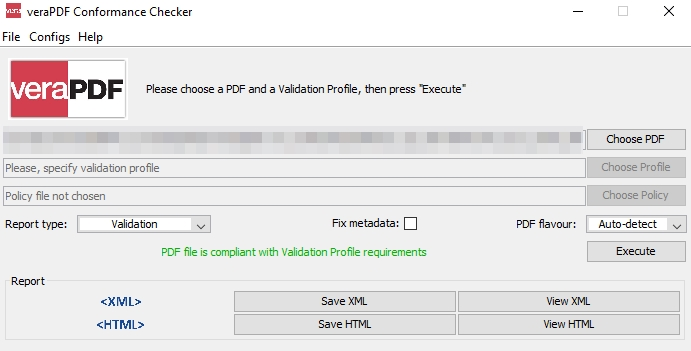
\includegraphics[height=100px]{./appendix/filesONLYForAppendix/Images/VeraPDF.jpg}
	\shadowimage[height=100px]{./zfiles/Bilder/VeraPDF.jpg}
	\caption{PDF-A Standard}
\end{figure}

\newpage

\label{a.1.pdf}
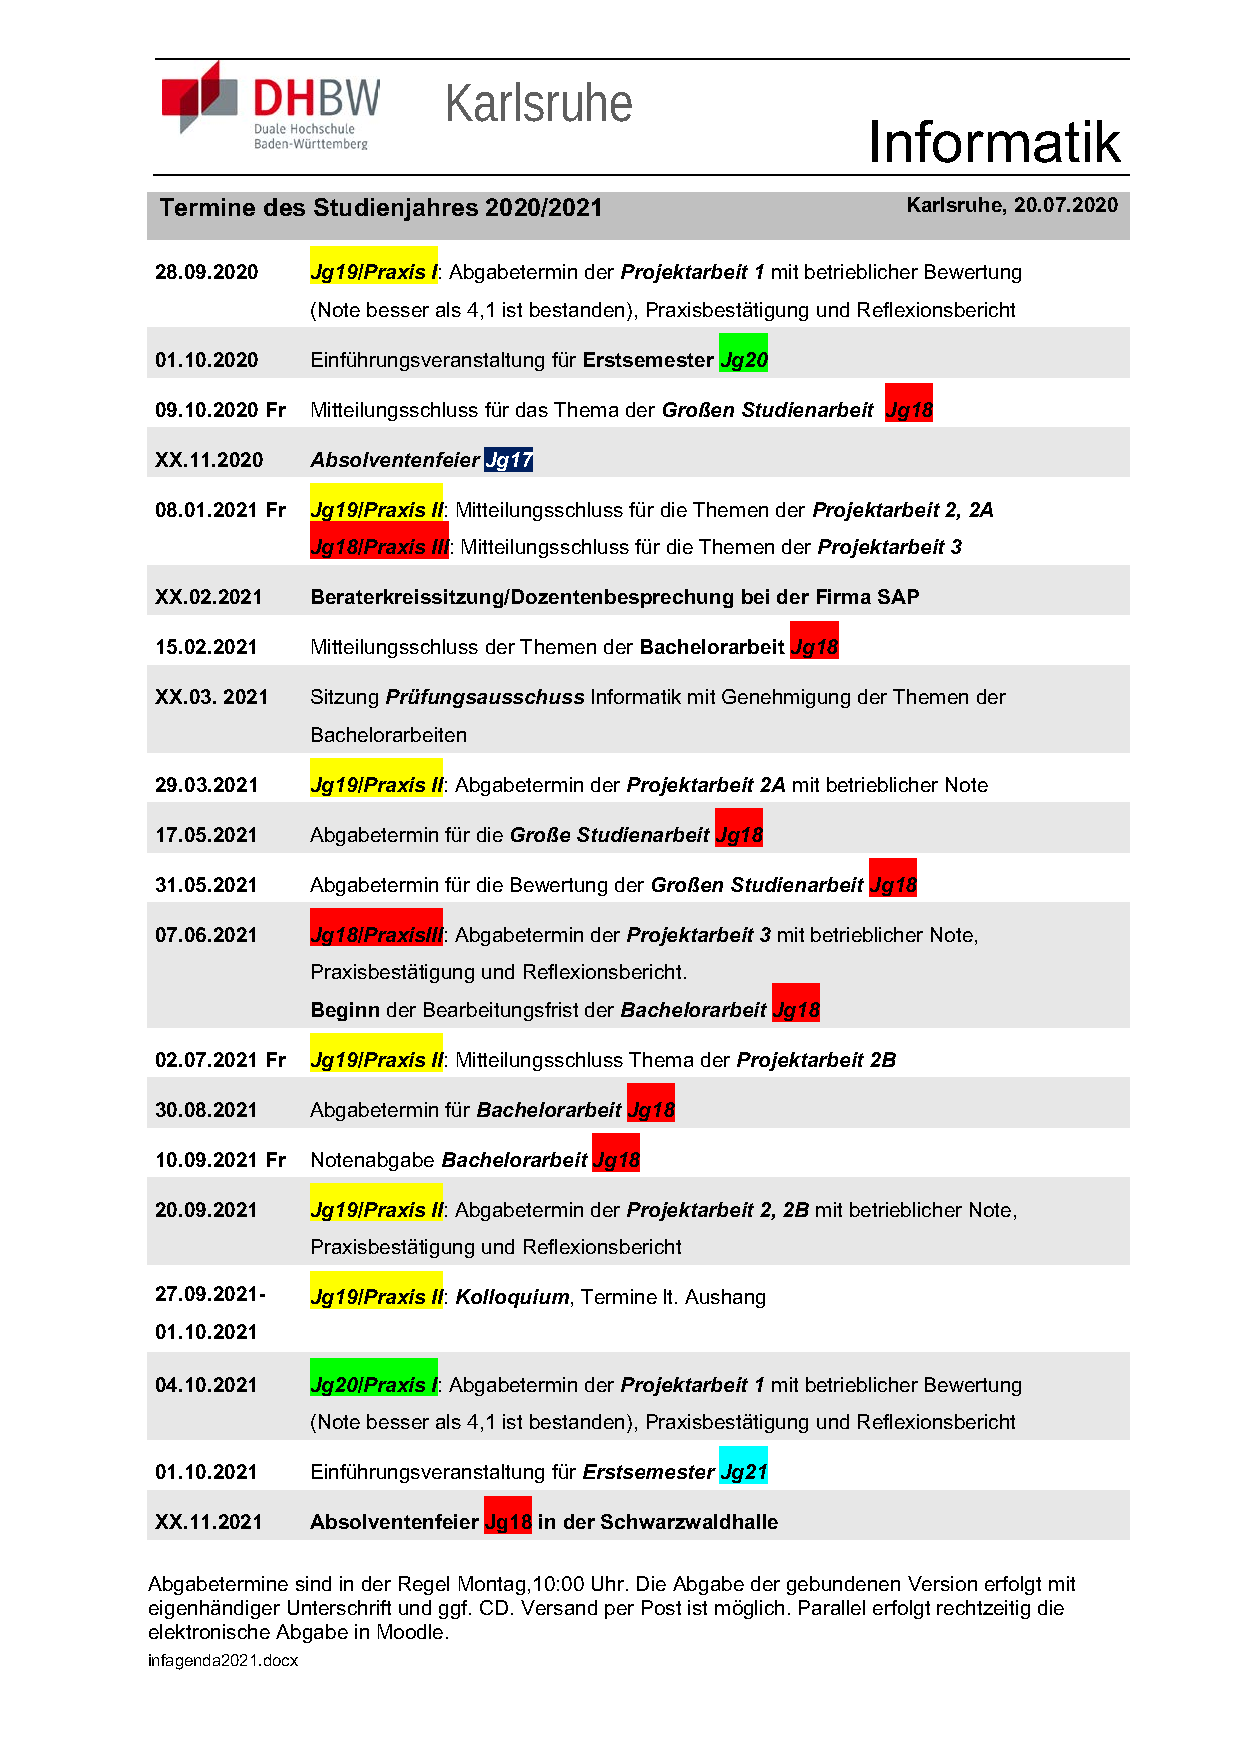
\includepdf[scale=0.7,pages=1,pagecommand=\section{PDF Include}]{./zfiles//Dokumente/infagenda2021}

\newpage

\section{SQL Snippet} \label{a.1.snippetSQL} 
\lstinputlisting[caption={SQL - Snippet},
					language=sql,
					frame = trBL]{./zfiles//Code/SQL/sqlSnippet.sql}

\newpage

\section{Java Snippet} \label{a.1.snippetJAVA} 
\lstinputlisting[caption={Java - Snippet},
language=sql,frame = trBL]{./zfiles/Code/Java/javaSnippet.java}

\newpage
%Beispiele für TiKZ Pictures , sind aber nich PDF-A Konform :(
%======================================================================
%	
%	                _                       
%	    /\         | |                      
%	   /  \   _ __ | |__   __ _ _ __   __ _ 
%	  / /\ \ | '_ \| '_ \ / _` | '_ \ / _` |
%	 / ____ \| | | | | | | (_| | | | | (_| |
%	/_/    \_\_| |_|_| |_|\__,_|_| |_|\__, |
%								       __/ |
%									  |___/ 
%
%----------------------------------------------------------------------
% Descripton : Appendix 2
%======================================================================

\begin{landscape}
	\section{Tikz - ERD}
	Leider nicht PDF-A Compliant - Deshalb nur ein Bild ....
	%\thispagestyle{plain}
\label{a.2.figure}
\tikzset{
	every entity/.style = {top color=white,bottom color=blue!30,draw=blue!50!black!100,drop shadow},
	every attribute/.style = {top color=white, bottom color=yellow!20,
		draw=yellow, drop shadow},
	every relationship/.style ={top color=white, bottom color=red!20,
		draw=red!50!black!100, drop shadow},
	every edge/.style = {link},
	every isa/.style = {top color=white, bottom color=green!20,
		draw=green!50!black!100, drop shadow},
}
	\vspace*{\stretch{1}}
	\begin{figure}[h]
		\centering
		\begin{adjustbox}{max height=0.5\textwidth}
			\begin{tikzpicture}[node distance=1.5cm, every edge/.style={link}]
				\node[entity] (attribute) {Hehe};
				
				\node[isa] (isa) [below=1cm of attribute] {IS A} edge (attribute);
				
				\node[entity] 	(pcav) 		[below left = 4cm of isa] {a} edge (isa);
				\node[attribute] (pcav1) [above left=of pcav] {b} edge (pcav);
				\node[attribute] (pcav2) [above=of pcav] {c} edge (pcav);
				
				\node[relationship] (pcav-rd) [below = of pcav]{1:n} edge (pcav);
				\node[relationship] (pcav-rt) [below right = of pcav]{1:n} edge (pcav);
				\node[relationship] (pcav-rlt) [below left = of pcav]{1:n} edge (pcav);
				
				\node[entity] 	(mlav) 		[below right = 4cm of isa] {e} edge (isa);
				\node[attribute] (mlav1) [above right=of mlav] {f} edge (mlav);
				\node[attribute] (mlav2) [above=of mlav] {g} edge (mlav);
				
				\node[relationship] (mlav-rd) [below = of mlav]{1:n} edge (mlav);
				\node[relationship] (mlav-rt) [below right = of mlav]{1:n} edge (mlav);
				\node[relationship] (mlav-rlt) [below left = of mlav]{1:n} edge (mlav);
				
				\node[entity] 	(t-double) 	[below  = 8cm of isa] {ms} edge (pcav-rd) edge (mlav-rd);
				\node[attribute] (d1) [below=of t-double,yshift=-1cm,xshift=1.7cm] {\key{h}} edge (t-double);
				\node[attribute] (d2) [below left =of t-double] {\key{i}} edge (t-double);
				\node[attribute] (d3) [below right=of t-double] {\key{j}} edge (t-double);
				\node[attribute] (d4) [below=of t-double,yshift=-1cm,xshift=-1.7cm] {k} edge (t-double);
				
				
				\node[entity] 	(t-text) 		[right = 8cm of t-double] {l} edge (pcav-rt) edge (mlav-rt);
				\node[attribute] (l1) [below=of t-text] {\key{n}} edge (t-text);
				\node[attribute] (l2) [below left =of t-text] {\key{o}} edge (t-text);
				\node[attribute] (l3) [below right=of t-text] {\key{p}} edge (t-text);
				\node[attribute] (l4) [right=of t-text] {textvalue} edge (t-text);
				
				\node[entity] 	(t-longtext) 	[left = 8cm of t-double] {ts} edge (pcav-rlt) edge (mlav-rlt);
				\node[attribute] (l1) [below=of t-longtext] {\key{q}} edge (t-longtext);
				\node[attribute] (l2) [below left =of t-longtext] {\key{r}} edge (t-longtext);
				\node[attribute] (l3) [below right=of t-longtext] {\key{s}} edge (t-longtext);
				\node[attribute] (l4) [left=of t-longtext] {z} edge (t-longtext);
				
			\end{tikzpicture}	
		\end{adjustbox}
	\caption{Entwurf eines ERD für die neue Datenstruktur}
	\end{figure}
\vspace{1cm}
	\begin{itemize}
		\item 1
		\item 2
	\end{itemize}
	
	\vspace{\stretch{1}}
	\begin{figure}[h]
		\centering
		\shadowimage[height=300px]{./zfiles/Bilder/ERD}
		\caption{Entwurf eines ERD für die Datenstruktur}
	\end{figure}
\end{landscape}

\newpage

\section{Tikz - Gantt-Diagramm} \label{a.2.gantt}
Leider nicht PDF-A Compliant - Deshalb nur ein Bild ....
\begin{figure}[h]
	\centering
	\shadowimage[height=450px]{./zfiles/Bilder/GANTT}
	\caption{Gantt Diagramm des Projektablaufs der 2. Praxisphase}
\end{figure}
%%%%%%%%%%%%%%%%%%%%%%%%%%%%%%%%%%%%%%%%%%%%%%%%%%%%%%%%%%%%%%%%%%%%%%%%%%%%%%%%
%% Descr:       Zusätzliche Befehler für das GANTT Diagramm
%% Author:      Nico Holzhäuser
%% -*- coding: utf-8 -*-
%%%%%%%%%%%%%%%%%%%%%%%%%%%%%%%%%%%%%%%%%%%%%%%%%%%%%%%%%%%%%%%%%%%%%%%%%%%%%%%

%TO BE UPDATED ACCORDING TO YOUR NEEDS
\def\mystartdate{2020-08-03}%starting date of the calendar
\def\myenddate{2020-09-28}%ending date of the calendar
\def\myxunit{.5cm}%width of 1 day
\def\myyunittitle{.5cm}%height of 1 title line
\def\myyunitchart{1cm}%height of 1 chart line

\def\pgfcalendarweekdayletter#1{% define the name of weekdays + formatting
    \ifcase#1M\or T\or W\or T\or F\or \textcolor{red!50!white}{S}\or \textcolor{red}{\textbf{S}}\fi
}   

%Some calculation for plotting week-ends area
    \newcount\myenddatecount
        \pgfcalendardatetojulian{\myenddate}{\myenddatecount}

    \newcount\mystartdatecount
        \pgfcalendardatetojulian{\mystartdate}{\mystartdatecount}

    \newcount\mynumberofdays
        \mynumberofdays \myenddatecount\relax
        \advance \mynumberofdays by -\mystartdatecount\relax% so \mynumberofdays is now the number of days in the calendar

    \newcount\mynumberofweeks
        \mynumberofweeks\mynumberofdays\relax
        \advance \mynumberofweeks by -1\relax
        \divide \mynumberofweeks by 7\relax% so we have the number of full weeks

    \newcount\myfirstweekday
        \pgfcalendarjuliantoweekday{\mystartdatecount}{\myfirstweekday}

    \newcount\myfirstweekendshift
        \myfirstweekendshift 5\relax
        \advance\myfirstweekendshift by -\myfirstweekday\relax
        \ifnum \myfirstweekendshift=-1%if first day = sunday
            \advance \myfirstweekendshift by 7\relax% the first full weekend will thus begin one week after
        \fi

\newpage

\section{Tikz - Graph} \label{a.2.graph1}
\begin{figure}[h!]
	\begin{center}
	
	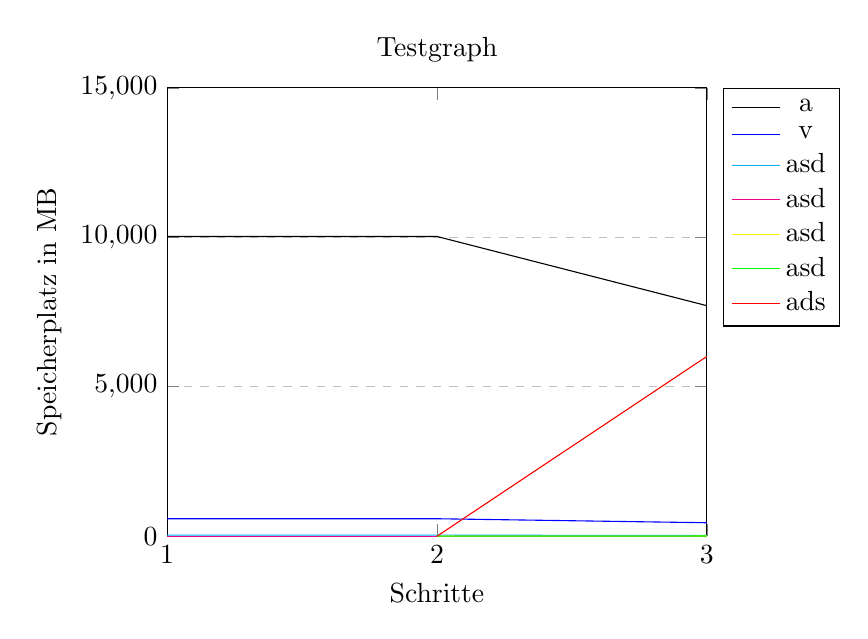
\begin{tikzpicture}
		\pgfplotsset{compat=1.12}
		\begin{axis}[
			title={Testgraph},
			xlabel={Schritte},
			ylabel={Speicherplatz in MB},
			xmin=1, xmax=3,
			ymin=0, ymax=15000,
			xtick={1,2,3},
			ytick={0,5000,10000,15000},
			yticklabel style={
				/pgf/number format/fixed,
				/pgf/number format/precision=5
			},
			scaled y ticks=false,
			legend pos=outer north east,
			ymajorgrids=true,
			grid style=dashed,
			]
			
			\addplot[
				color=black,
				]
				coordinates {
					(1,10028)(2,10028)(3,7713)
				};\label{g-s-1}
			
			\addplot[
			color=blue,
			]
			coordinates {
				(1,584)(2,584)(3,450)
			};\label{g-s-2}
		
			\addplot[
			color=cyan,
			]
			coordinates {
				(1,34)(2,34)(3,23)
			};\label{g-s-3}
		
			\addplot[
			color=magenta,
			]
			coordinates {
				(1,0.02)(2,0.02)(3,0.02)
			};\label{g-s-4}
		
			\addplot[
			color=yellow,
			]
			coordinates {
				(2,0)(3,4.84)
			};\label{g-s-5}
		
			\addplot[
			color=green,
			]
			coordinates {
				(2,0)(3,4.911)
			};\label{g-s-6}
		
			\addplot[
			color=red,
			]
			coordinates {
				(2,0)(3,6013)
			}; \label{g-s-7}
			\addlegendimage{/pgfplots/refstyle=g-s-1}\addlegendentry{a}
			\addlegendimage{/pgfplots/refstyle=g-s-2}\addlegendentry{v}
			\addlegendimage{/pgfplots/refstyle=g-s-3}\addlegendentry{asd}
			\addlegendimage{/pgfplots/refstyle=g-s-4}\addlegendentry{asd}
			\addlegendimage{/pgfplots/refstyle=g-s-5}\addlegendentry{asd}
			\addlegendimage{/pgfplots/refstyle=g-s-6}\addlegendentry{asd}
			\addlegendimage{/pgfplots/refstyle=g-s-7}\addlegendentry{ads}
		\end{axis}
	\end{tikzpicture}
	\end{center}
	\caption{Speicherplatz der Tabellen}
\end{figure}

\newpage

\section{Tabelle} \label{a.2.graph2}
\begin{table}[h]
	\centering
	\begin{tabular}{|c|r|r|r|}
		\hline
		\multicolumn{1}{|c|}{Tabelle} & \multicolumn{1}{c|}{1} & \multicolumn{1}{c|}{2} & \multicolumn{1}{c|}{3}	\\
		\hline
		Hallo   	& 	   0,00 MB 		& 3,00 MB 		&  2,00 MB 		\\
		Hallo   	& 	   0,00 MB 		& 3,00 MB 		&  2,00 MB 		\\
		Hallo   	& 	   0,00 MB 		& 3,00 MB 		&  2,00 MB 		\\
		Hallo   	& 	   0,00 MB 		& 3,00 MB 		&  2,00 MB 		\\
		Hallo   	& 	   0,00 MB 		& 3,00 MB 		&  2,00 MB 		\\
		Hallo   	& 	   0,00 MB 		& 3,00 MB 		&  2,00 MB 		\\
		Hallo   	& 	   0,00 MB 		& 3,00 MB 		&  2,00 MB 		\\
		\hline
		Gesamt								& 0,02 MB		& \cellcolor{yellow!25} + 0,02 MB		&  \cellcolor{red!25} + 0,86 MB		\\
		\hline
	\end{tabular}
	\caption{Speicherplatzveränderung}
\end{table}

	\cleardoublepage
	\ifthenelse{\boolean{DEBUG}}{}{\cleardoublepage}
	
	%—————————————————————————————————————————————————————————————————————————
	%						Index
	%—————————————————————————————————————————————————————————————————————————
	\ifthenelse{\boolean{INDEX}}{
		\phantomsection
		\addcontentsline{toc}{chapter}{Index}
		\printindex
	}{}
	\ifthenelse{\boolean{DEBUG}}{}{\cleardoublepage}
	
	%—————————————————————————————————————————————————————————————————————————
	%						Literaturverzeichnis
	%—————————————————————————————————————————————————————————————————————————
	\ifthenelse{\boolean{LITERATURVERWEIS}}{\renewcommand\bibname{Literaturverzeichnis \\ \vspace{10mm} \normalsize{} Alle Quellen sind zusätzlich im Ordner \HREF{./Quellensicherung}{Quellensicherung} gespeichert ! \vspace{-2cm}}}{\def\refname{Literaturverzeichnis}}
	\phantomsection
	\addcontentsline{toc}{chapter}{Literaturverzeichnis}
	\printbibliography
	\ifthenelse{\boolean{DEBUG}}{}{\cleardoublepage}
	
	%—————————————————————————————————————————————————————————————————————————
	%						Inhaltsbeilage
	%—————————————————————————————————————————————————————————————————————————
	% Für Sophia auch noch ein Inhaltsverzeichnis ;)
	\cleardoublepage
	\ifthenelse{\boolean{DOKUMENTENVERZEICHNIS}}{
		\cleardoublepage

\pagestyle{empty}

\chapter*{Dokumentenverzeichnis}
In diesem Umschlag befinden sich folgende Dokumente :
\begin{itemize}
	\item \fett{Dokumentenverzeichnis}
	\begin{itemize}
		\item \fett{einzelne} Seite(n)
	\end{itemize}
	\item \fett{\Was} - \Titel
	\begin{itemize}
		\item \fett{\theTotPages} Seite(n)
	\end{itemize}
	\item \fett{Bewertung der \Was}
	\begin{itemize}
		\item \fett{drei} Seite(n)
	\end{itemize}
	\item \fett{Praxisbericht Teil A}
	\begin{itemize}
		\item \fett{einzelne} Seite(n)
	\end{itemize}
	\item \fett{Praxisbericht Teil B}
	\begin{itemize}
		\item \fett{einzelne} Seite(n)
	\end{itemize}
	\ifthenelse{\boolean{CDBEILAGE}}{
		\item \fett{Dateisicherung}
			\begin{itemize}
				\item \fett{eine} CD, befestigt im \textbf{hinteren} Teil des Umschlages der \\ \Was
			\end{itemize}
	}{}
\end{itemize}

% https://golatex.de/viewtopic.php?t=15622
\vspace{4cm}
\noindent\rule{5cm}{.4pt}\hfill\rule{5cm}{.4pt}\par
\noindent Datum, Ort \hfill Unterschrift
		\pagebreak
	}{}
	\ifthenelse{\boolean{DATEIVERZEICHNIS}}{
		\cleardoublepage

\pagenumbering{gobble}
\pagestyle{plain}

\chapter*{Dateiverzeichnis}
In dieser Dateistruktur befinden sich folgende Dokumente und Dateien :
\begin{itemize}
	\item \fett{Dateiverzeichnis} - \HREF{./Dateiverzeichnis.pdf}{Dateiverzeichnis.pdf}	
	\item \fett{\Was} - \Titel --  \HREF{./ProjektArbeit_Typ_Martrikelnummer_Kurs_Name.pdf}{ProjektArbeit\_Typ\_Martrikelnummer\_Kurs\_Name.pdf}
	\item \fett{Quellensicherung} - \HREF{Quellensicherung}{./Quellensicherung}
	\item \fett{Quellcode} -  \HREF{Quellcode}{./Quellcode}
	\item \fett{Praxisbericht Teil A - Ablauf der Praxisphase} - \HREF{./Berichte/Teil-A.pdf}{./Berichte/Teil-A.pdf}
	\item \fett{Praxisbericht Teil B - Reflexionsbericht} - \HREF{./Berichte/Teil-B.pdf}{./Berichte/Teil-B.pdf}
	\item \fett{Bewertung der \Was} - \HREF{./Berichte/Bewertung.pdf}{./Berichte/Bewertung.pdf}
\end{itemize}

% https://golatex.de/viewtopic.php?t=15622
%\vspace{5cm}
%\noindent\rule{5cm}{.4pt}\hfill\rule{5cm}{.4pt}\par
%\noindent Datum, Ort \hfill Unterschrift

\vspace{8cm}
Seite \fett{1} von \fett{1}
		\pagebreak
	}{}
	
	%—————————————————————————————————————————————————————————————————————————
	%								Oranisatorisches
	%—————————————————————————————————————————————————————————————————————————
	\ifthenelse{\boolean{BERICHTE}}{
		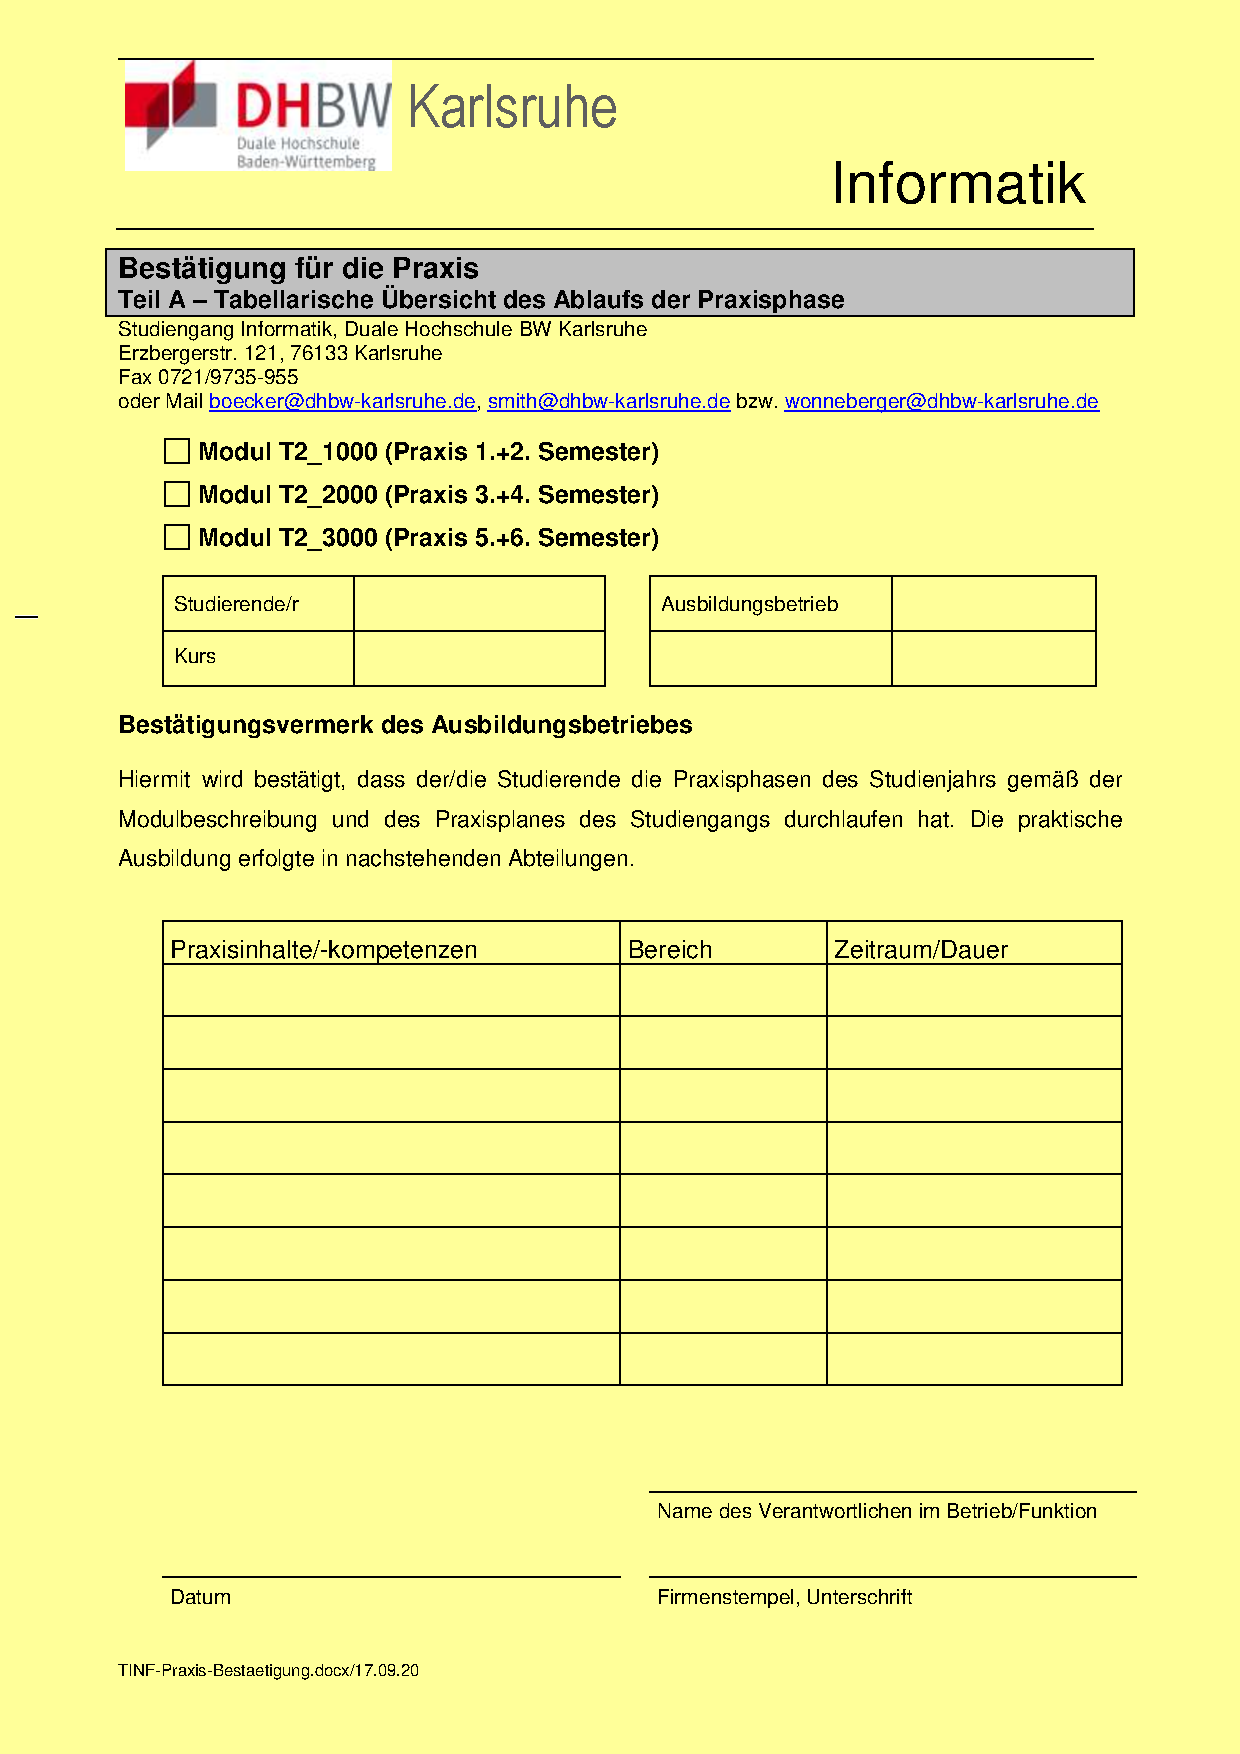
\includepdf[fitpaper=true, pages=1]{./zfiles/Dokumente/Teil-A}
		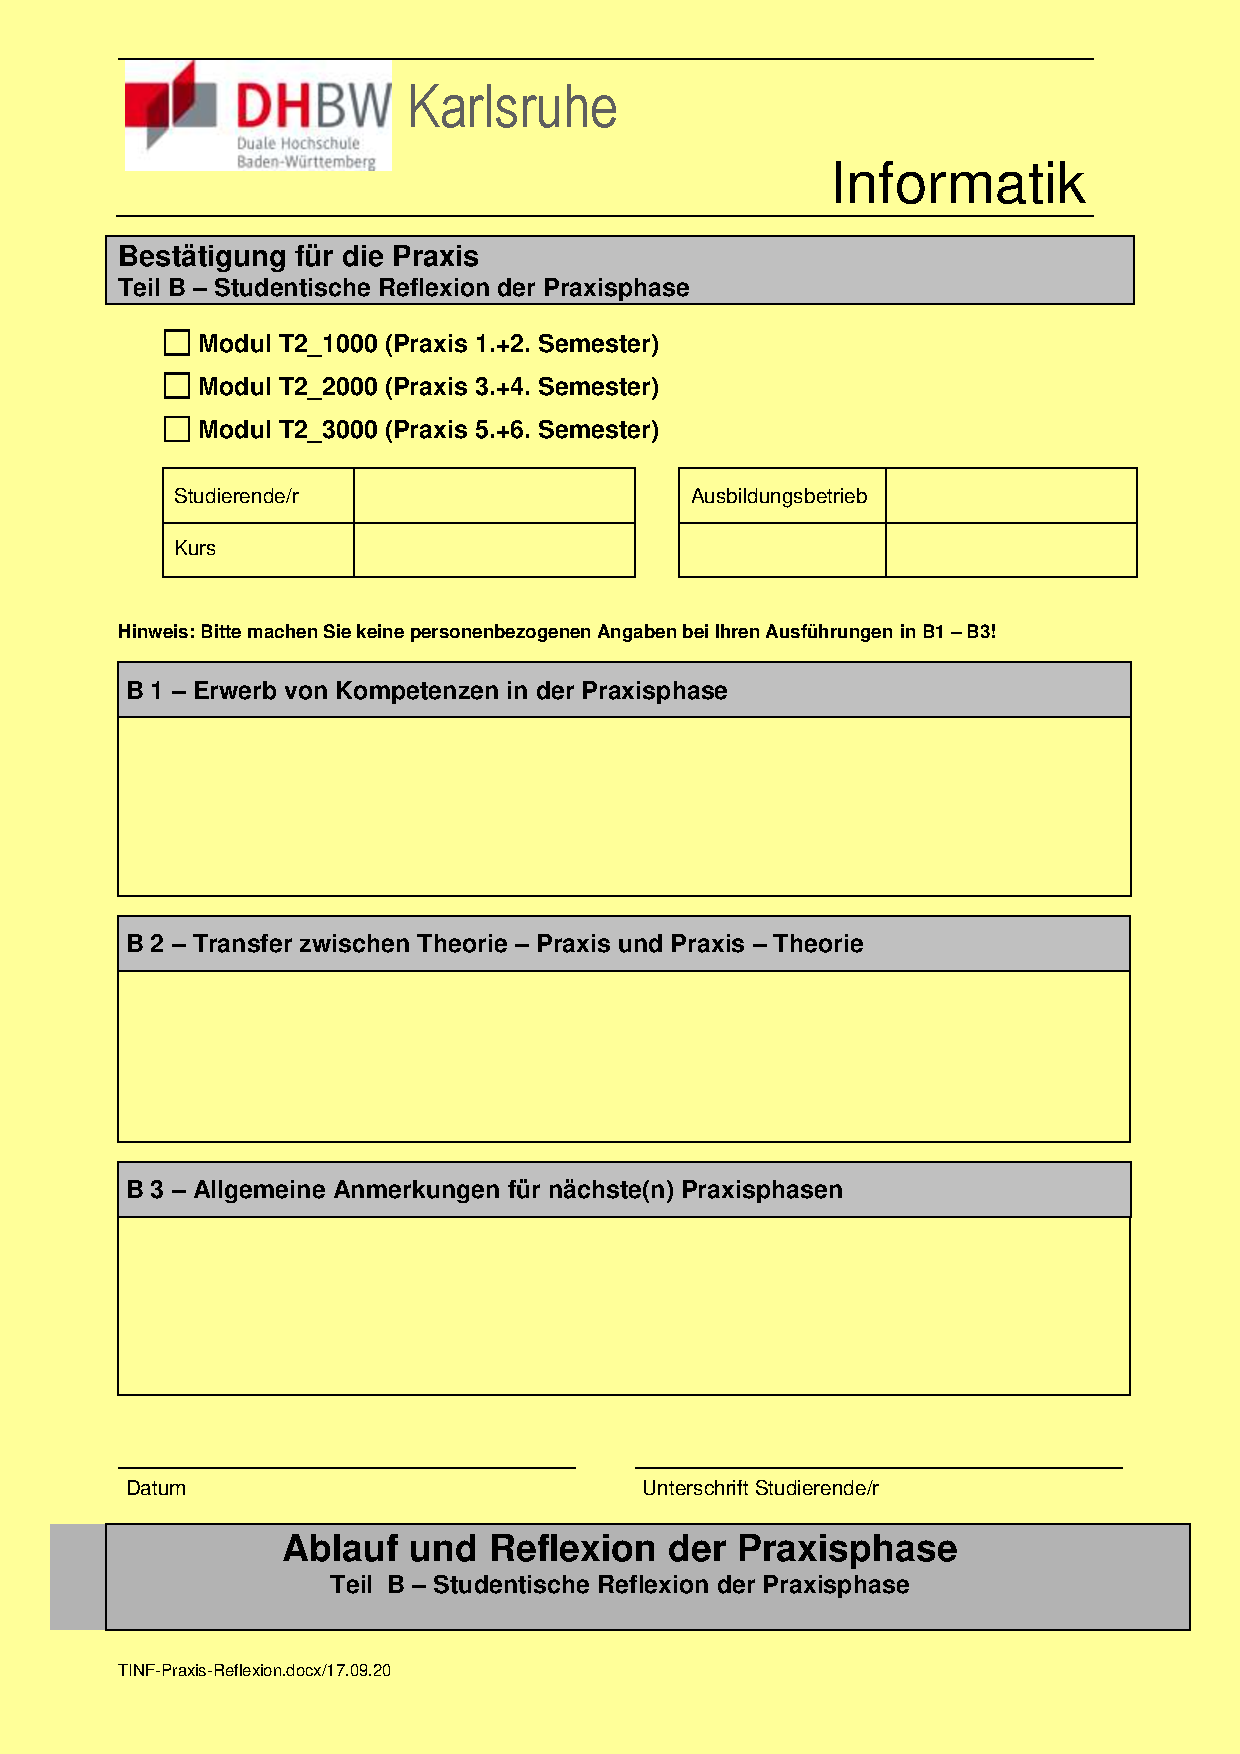
\includepdf[fitpaper=true, pages=1]{./zfiles/Dokumente/Teil-B}
		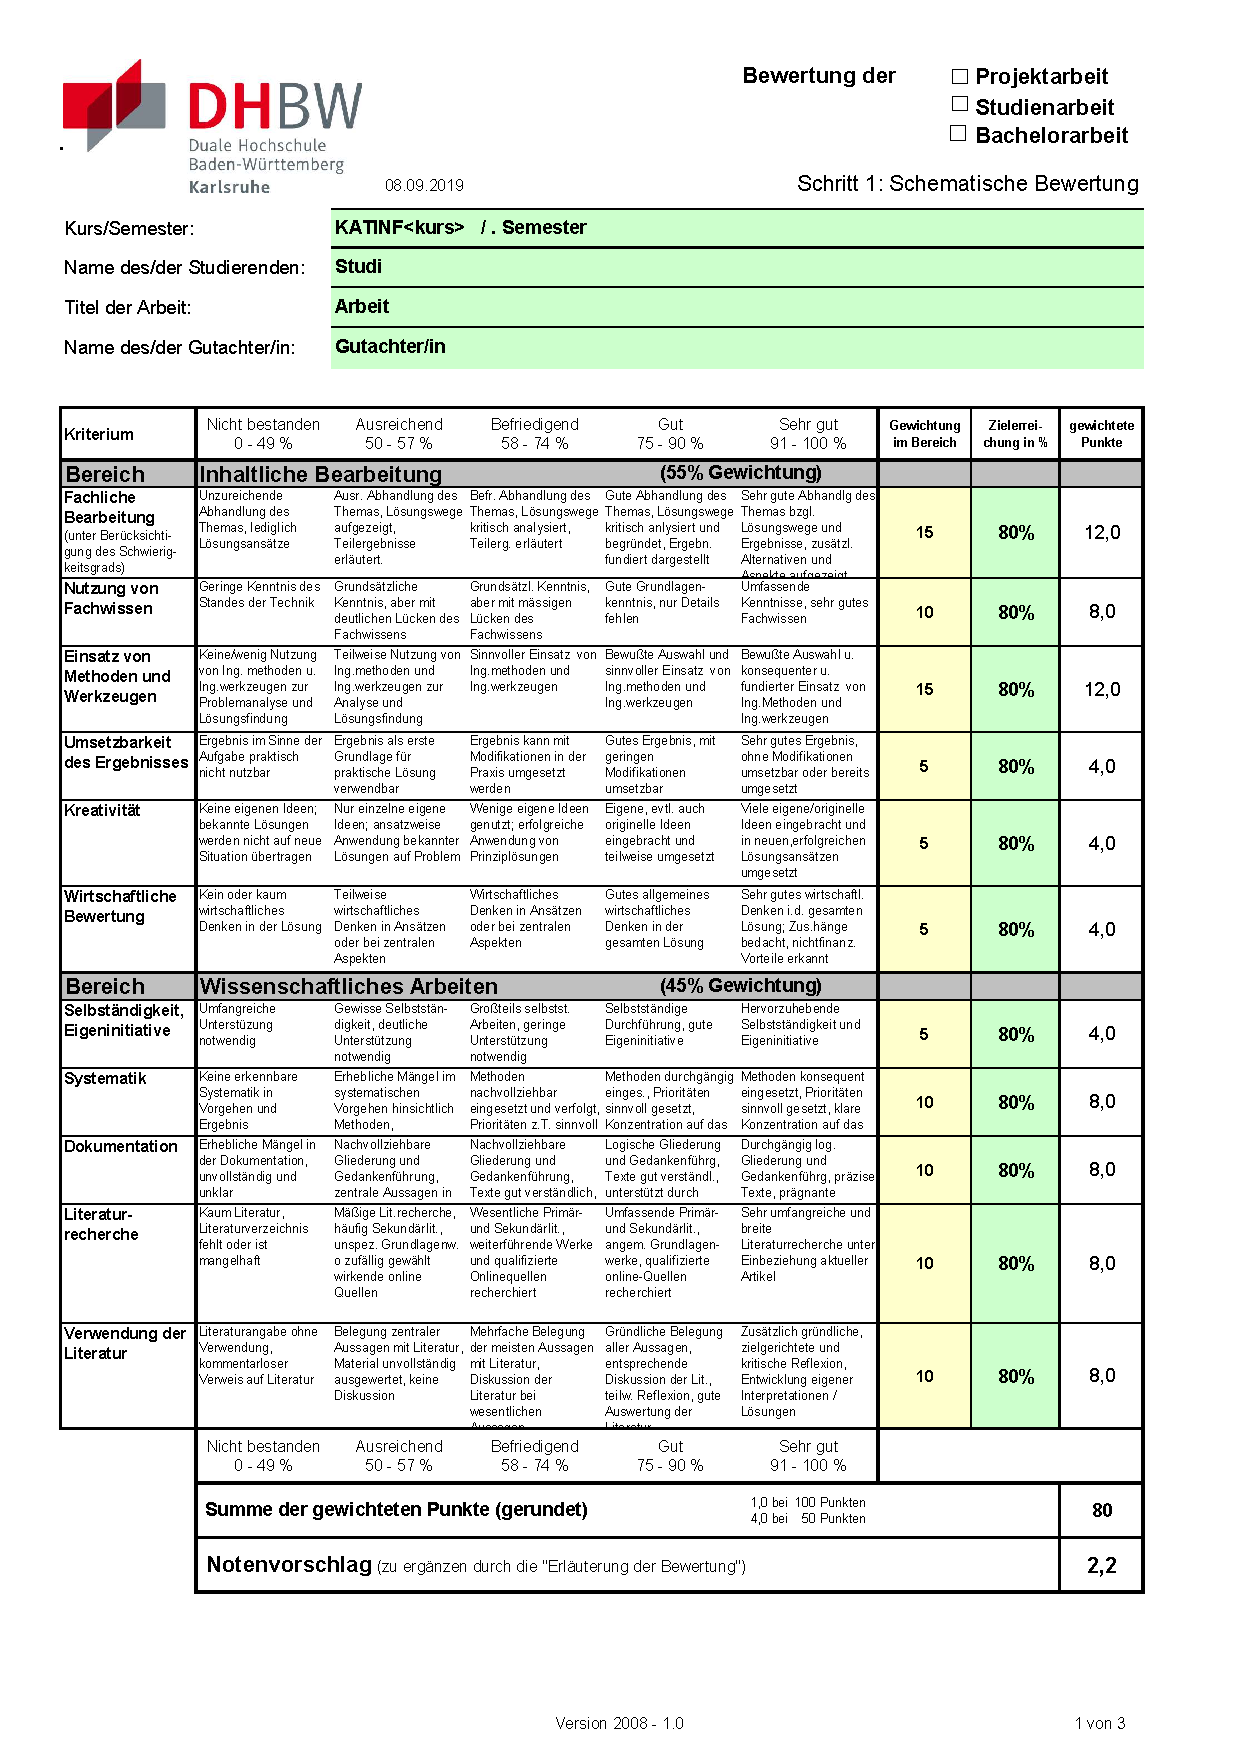
\includepdf[fitpaper=true, pages=1-3]{./zfiles/Dokumente/Bewertung}
	}{} 
	
	\ifthenelse{\boolean{DEBUG}}{}{\cleardoublepage}
\end{document}
